\فصل{درخت‌های عمومی، دودویی و هیپ}

\قسمت{مقدمه}

داده‌ساختار درخت یکی از مهمترین و کاربردی‌ترین داده‌ساختارها است. انواع مختلفی از این داده‌ساختار وجود دارد و سوالات مطرح شده در این فصل تنها بخش کوچکی از این انواع را پوشش می‌دهد. 

داده‌ساختار درخت کاربردهای فراوانی در علم کامپیوتر دارد که از جمله کاربردهای آن می‌توان به پیاده‌سازی سیستم فایل‌های سلسله مراتبی اشاره کرد مانند آنچه در سیستم عامل ویندوز یا گنو/لینوکس وجود دارد. همچنین شالوده‌ی سامانه‌ی نام دامنه\پانویس{{\lr{Domain Name System (DNS)}}} از ساختار درختی پیروی می‌کند.

با توجه به اینکه برای برخی از مفاهیم داده‌ساختار درخت، مانند سطح، عمق، ارتفاع و غیره، در کتاب‌های مرجع تعاریف مختلفی ارائه شده است در ادامه تعاریفی که از آنها در این فصل استفاده شده است آورده خواهد شد.

\متن‌سیاه{سطح\پانویس{{\lr{Level}}} یک گره}: سطح گره {$x$} برابر است با تعداد یال‌هایی که باید از گره ریشه طی کرد تا به گره {$x$} رسید بعلاوه یک. به این ترتیب گره ریشه دارای سطح یک است، فرزندان ریشه دارای سطح دو هستند و به همین ترتیب.

\متن‌سیاه{عمق\پانویس{{\lr{Depth}}} یک گره}: عمق گره {$x$} برابر است با تعداد یال‌هایی که باید از گره ریشه طی کرد تا به گره {$x$} رسید. در این صورت گره ریشه دارای عمق صفر است، فرزندان ریشه دارای عمق یک هستند و به همین ترتیب. عمق درخت {$T$} برابر با عمق عمیق‌ترین گره درخت {$T$} است.

\متن‌سیاه{ارتفاع\پانویس{{\lr{Height}}} یک گره}: ارتفاع گره {$x$} برابر است با تعداد یالهای طولانی‌ترین مسیری که گره {$x$} را به یک گره برگ متصل می‌کند. با این تعریف می‌توان نتیجه گرفت تمام گره‌های برگ در یک درخت دارای ارتفاع صفر هستند. ارتفاع درخت {$T$} برابر با ارتفاع ریشه آن است.

\متن‌سیاه{درخت {$\mathbf{k}$}تایی پر}: درخت {$T$} یک درخت {$k$}تایی پر است اگر تمام گره‌های غیر برگ آن دارای دقیقا {$k$} فرزند باشند و همچنین تمام گره‌های برگ آن در یک سطح قرار گرفته باشند.

\متن‌سیاه{ساختار گره‌ی درخت دودویی}: ساختار گره‌ی یک درخت دودویی دارای سه فیلد {\id{data}}، {\id{leftChild}} و {\id{rightChild}} است که از اولین فیلد برای نگهداری مقدار داده‌ای و از فیلدهای دوم و سوم به ترتیب برای اشاره به فرزند چپ و راست گره استفاده می‌شود.

\متن‌سیاه{ساختار گره‌ی درخت عمومی}: ساختار گره‌ی یک درخت عمومی دارای سه فیلد {\id{data}}، {\id{next}} و {\id{children}} است که از فیلد اول برای نگهداری مقدار داده‌ای، از فیلد دوم برای اشاره به همنیای سمت راست و از فیلد سوم برای اشاره به لیست فرزندان گره استفاده می‌شود.

\قسمت{منابع مطالعاتی}

برای مطالعه در مورد تعاریف و فرمول‌های درخت و همچنین درخت‌های عمومی و دودویی می‌توانید به فصل هفتم {\cite{ebrahimi}} و فصل پنجم {\cite{horowitz}} مراجعه کنید. برای کسب اطلاعات در مورد درخت‌های هیپ فصل نهم {\cite{ebrahimi}} و فصل ششم {\cite{weiss}} منابع مناسبی هستند.

\قسمت{فرمول‌های درخت}

\سوال ثابت کنید عمق یک درخت {$k$}تایی پر با {$n$} گره، برابر با {$\lfloor \log_k n \rfloor$} است.

\پاسخ

در عمق صفر یک درخت {$k$}تایی پر دارای تنها یک گره هستیم که همان گره‌ی ریشه است. در عمق یک چنین درختی دارای {$k$} گره خواهیم بود زیرا درخت پر است و گره ریشه باید دارای دقیقاً {$k$} فرزند باشد. در عمق دو دارای {$k^2$} گره خواهیم بود و به همین ترتیب. به عبارت بهتر تعداد گره‌ها در عمق {$d$} ({$d \neq 0$})، {$k$} برابر تعداد گره‌های عمق {$d-1$} است. برای درک بهتر این موضوع به شکل {\eqref{ch5:fig:kAryFullTree}} توجه کنید.

\begin{figure}[H]
\begin{center}
\scalebox{0.9}
{
\begin{pspicture}(0,-2.355)(9.5275,2.375)
\pscircle[linewidth=0.04,dimen=outer](3.65,1.235){0.41}
\pscircle[linewidth=0.04,dimen=outer](5.91,0.135){0.41}
\pscircle[linewidth=0.04,dimen=outer](1.57,0.135){0.41}
\psline[linewidth=0.04cm](3.3,1.025)(1.84,0.425)
\psline[linewidth=0.04cm](4.0,1.045)(5.66,0.425)
\pscircle[linewidth=0.04,dimen=outer](2.41,-1.065){0.41}
\pscircle[linewidth=0.04,dimen=outer](0.71,-1.045){0.41}
\psline[linewidth=0.04cm](1.28,-0.135)(0.76,-0.655)
\psline[linewidth=0.04cm](1.84,-0.135)(2.36,-0.675)
\psline[linewidth=0.04cm,linestyle=dotted,dotsep=0.16cm](2.92,0.105)(4.44,0.105)
\psline[linewidth=0.04cm,linestyle=dotted,dotsep=0.16cm](3.16,-1.075)(4.34,-1.055)
\psline[linewidth=0.04cm,linestyle=dashed,dash=0.16cm 0.16cm](0.46,-1.355)(0.0,-2.075)
\psline[linewidth=0.04cm,linestyle=dashed,dash=0.16cm 0.16cm](0.94,-1.355)(1.38,-2.075)
\psline[linewidth=0.04cm,linestyle=dotted,dotsep=0.16cm](1.36,-1.055)(1.8,-1.055)
\usefont{T1}{ptm}{m}{n}
\rput(3.626875,1.255){$1$}
\rput(1.5785937,0.155){$1$}
\rput(5.909531,0.175){$k$}
\rput(7.732969,2.135){\rl{عمق}}
\rput(7.7370315,1.235){$0$}
\rput(7.706875,0.155){$1$}
\rput(7.7385936,-1.025){$2$}
\rput(9.072657,2.195){\rl{تعداد گره}}
\rput(0.70765626,-1.045){$1$}
\rput(6.7509375,-1.045){$k^2$}
\rput(9.112031,1.275){$k^0$}
\rput(9.056406,0.155){$k^1$}
\rput(9.070937,-1.005){$k^2$}
\psline[linewidth=0.04cm,linestyle=dotted,dotsep=0.16cm](7.76,-1.535)(7.76,-2.335)
\psline[linewidth=0.04cm,linestyle=dotted,dotsep=0.16cm](9.02,-1.535)(9.02,-2.335)
\psline[linewidth=0.04cm,linestyle=dashed,dash=0.16cm 0.16cm](2.18,-1.355)(1.72,-2.075)
\psline[linewidth=0.04cm,linestyle=dashed,dash=0.16cm 0.16cm](2.68,-1.355)(3.12,-2.075)
\pscircle[linewidth=0.04,dimen=outer](6.73,-1.065){0.41}
\pscircle[linewidth=0.04,dimen=outer](5.03,-1.045){0.41}
\psline[linewidth=0.04cm](5.62,-0.135)(5.1,-0.655)
\psline[linewidth=0.04cm](6.16,-0.175)(6.66,-0.675)
\psline[linewidth=0.04cm,linestyle=dashed,dash=0.16cm 0.16cm](4.78,-1.355)(4.32,-2.075)
\psline[linewidth=0.04cm,linestyle=dashed,dash=0.16cm 0.16cm](5.26,-1.355)(5.7,-2.075)
\psline[linewidth=0.04cm,linestyle=dotted,dotsep=0.16cm](5.68,-1.055)(6.12,-1.055)
\psline[linewidth=0.04cm,linestyle=dashed,dash=0.16cm 0.16cm](6.5,-1.355)(6.04,-2.075)
\psline[linewidth=0.04cm,linestyle=dashed,dash=0.16cm 0.16cm](7.0,-1.355)(7.44,-2.075)
\end{pspicture} 
}\caption{بخشی از یک درخت {$k$}تایی پر}\label{ch5:fig:kAryFullTree}
\end{center}
\end{figure}

با در نظر گرفتن شکل {\eqref{ch5:fig:kAryFullTree}} تعداد کل گره‌ها، که آن را با {$n$} نمایش می‌دهیم، در یک درخت {$k$}تایی پر به عمق {$m$} به صورت زیر به دست می‌آید:
\begin{align}
n &= 1+k+k^2+k^3+\cdots + k^m\nonumber\\
   &=\frac{k^{m+1}-1}{k-1}\label{ch5:eqn:nNodes}
\end{align}
اگر در عبارت {$\lfloor \log_k n \rfloor$} به جای {$n$}، مقدار به دست آمده از {\eqref{ch5:eqn:nNodes}} را قرار دهیم باید داشته باشیم:
\begin{equation}
\left\lfloor \log_k \frac{k^{m+1}-1}{k-1} \right\rfloor=m\label{ch5:eqn:treeHeight}
\end{equation}
به این ترتیب باید ثابت کنیم تساوی {\eqref{ch5:eqn:treeHeight}} برقرار است. در ادامه، به اثبات برقراری این تساوی می‌پردازیم.

با در نظر گرفتن خاصیت تابع جزء صحیح می‌توان تساوی {\eqref{ch5:eqn:treeHeight}} را به صورت زیر نوشت:
\begin{equation}
m \leq \log_k \frac{k^{m+1}-1}{k-1} < m+1\label{ch5:eqn:treeHeightIneq1}
\end{equation}
اگر طرفین نامعادله {\eqref{ch5:eqn:treeHeightIneq1}} را به عنوان توان عدد {$k$} در نظر بگیریم خواهیم داشت:
\begin{equation}
k^m \leq k^{\log_k \frac{k^{m+1}-1}{k-1}} < k^{m+1} \Rightarrow k^m \leq \frac{k^{m+1}-1}{k-1} < k^{m+1}\label{ch5:eqn:treeHeightIneq2}
\end{equation}

با ضرب طرفین نامعادله {\eqref{ch5:eqn:treeHeightIneq2}} در {$k-1$} داریم:
\begin{equation}
k^m(k-1) \leq k^{m+1}-1 < k^{m+1}(k-1)\label{ch5:eqn:treeHeightIneq3}
\end{equation}
با ساده‌سازی نامعادله {\eqref{ch5:eqn:treeHeightIneq3}} به عبارت زیر می‌رسیم:
\begin{equation}
k^{m+1}-k^m \leq k^{m+1}-1 < k^{m+1}(k-1)\label{ch5:eqn:treeHeightIneq4}
\end{equation}
درستی نامعادله {\ref{ch5:eqn:treeHeightIneq4}} را می‌توان با استقرا بر روی {$m$} نشان داد و اثبات را کامل کرد. انجام استقرا به خواننده واگذار می‌شود.

\سوال فرض کنید برای پیاده‌سازی درخت‌های {$k$}تایی از گره‌هایی با قالب نشان داده شده در شکل {\eqref{ch5:fig:treeNodeStruct}} استفاده شده است. در چنین ساختاری دارای یک فیلد داده‌ای و {$k$} فیلد اشاره‌گر برای اشاره به هر یک از {$k$} زیردرخت یک گره هستیم. اگر دارای {$n$} گره در چنین درختی باشیم آنگاه تعداد اشاره‌گرهای تهی چه تعداد خواهد بود؟
\begin{figure}[H]
\begin{center}
\scalebox{0.8}
{
\begin{pspicture}(0,-1.87)(12.255546,1.87)
\psframe[linewidth=0.04,dimen=outer](8.26,1.11)(4.06,0.31)
\psline[linewidth=0.04cm](4.86,1.07)(4.86,0.33)
\pstriangle[linewidth=0.04,dimen=outer](1.33,-1.87)(2.66,1.34)
\pstriangle[linewidth=0.04,dimen=outer](7.95,-1.87)(2.66,1.34)
\psframe[linewidth=0.04,dimen=outer](8.26,1.87)(4.06,1.07)
\usefont{T1}{ptm}{m}{n}
\rput(6.1545315,1.46){\rl{فیلد داده}}
\psdots[dotsize=0.14](4.46,0.73)
\psdots[dotsize=0.14](7.86,0.71)
\psline[linewidth=0.04cm,arrowsize=0.05291667cm 2.0,arrowlength=1.4,arrowinset=0.4]{->}(4.42,0.71)(1.38,-0.45)
\psline[linewidth=0.04cm,arrowsize=0.05291667cm 2.0,arrowlength=1.4,arrowinset=0.4]{->}(7.04,0.69)(7.96,-0.47)
\rput(1.33625,-1.34){$T_1$}
\rput(4.3907814,-1.34){$T_2$}
\rput(8.12625,-1.34){$T_{k-1}$}
\psline[linewidth=0.04cm,linestyle=dotted,dotsep=0.16cm](5.72,-1.07)(6.6,-1.07)
\pstriangle[linewidth=0.04,dimen=outer](4.35,-1.87)(2.66,1.34)
\psdots[dotsize=0.14](5.24,0.71)
\psline[linewidth=0.04cm,arrowsize=0.05291667cm 2.0,arrowlength=1.4,arrowinset=0.4]{->}(5.24,0.71)(4.4,-0.43)
\psline[linewidth=0.04cm](6.64,1.11)(6.64,0.33)
\psdots[dotsize=0.14](7.04,0.69)
\pstriangle[linewidth=0.04,dimen=outer](10.95,-1.87)(2.66,1.34)
\rput(10.999375,-1.34){$T_k$}
\psline[linewidth=0.04cm,arrowsize=0.05291667cm 2.0,arrowlength=1.4,arrowinset=0.4]{->}(7.84,0.73)(10.9,-0.47)
\psline[linewidth=0.04cm,linestyle=dotted,dotsep=0.16cm](5.88,0.73)(6.46,0.73)
\psline[linewidth=0.04cm](7.46,1.11)(7.46,0.33)
\psline[linewidth=0.04cm](5.66,1.11)(5.66,0.33)
\end{pspicture} 
}
\caption{ساختار یک گره در یک درخت {$k$}تایی}\label{ch5:fig:treeNodeStruct}
\end{center}
\end{figure}

\پاسخ

در چنین ساختاری هر گره دارای {$k$} اشاره‌گر است. در نتیجه هنگامی که {$n$} گره در درخت وجود دارد دارای {$nk$} اشاره‌گر هستیم. از این تعداد اشاره‌گر فقط {$n-1$} اشاره‌گر مورد استفاده قرار می‌گیرند زیرا برای اشاره به هر یک از گره‌ها به جز گره ریشه به یک اشاره‌گر نیاز است. اگر تعداد کل اشاره‌گرها را از تعداد اشاره‌گرهای مورد استفاده کم کنیم خواهیم داشت:
\begin{displaymath}
nk-(n-1)=nk-n+1=n(k-1)+1
\end{displaymath}
به این ترتیب تعداد اشاره‌گرهای تهی برابر با {$n(k-1)+1$} است.

\قسمت{درخت‌های عمومی و دودویی}

\سوال با فرض پیاده‌سازی درخت عمومی به کمک اشاره‌گرها و اینکه هر گره موظف است آدرس فرزندان خود را در یک لیست پیوندی نگاه دارد، تابعی بازگشتی بنویسید که بررسی کند آیا عنصری با مقدار {$x$} در درخت داده شده وجود دارد یا خیر. اگر {$x$} موجود بود مقدار {\const{true}} و در غیر اینصورت مقدار {\const{false}} به عنوان خروجی تابع برگردانده شود.

\پاسخ

شبه کد تابعی بازگشتی که در درخت {\id{gTree}} به دنبال عنصری با مقدار {$x$} می‌گردد در الگوریتم {\eqref{ch5:alg:findx}} آمده است. در ادامه به بررسی روش عملکرد این تابع پرداخته می‌شود.
\begin{algorithm}[H]
\caption{بررسی وجود عنصری با مقدار مشخص در یک درخت عمومی}\label{ch5:alg:findx}
\begin{latin}
\begin{algorithmic}[1]
\Function{Find}{$\id{gTree},x$}
		\If{$\id{gTree} \isequal \const{null}$}
				\State	\Return
		\EndIf
		\If{$\attrib{\id{gTree}}{\id{data}} \isequal x$}
				\State	\Return \const{true}
		\EndIf
		\State	$\id{found} \gets \const{false}$
		\State	$p \gets \attrib{\id{gTree}}{\id{children}}$
		\While{$p \neq \const{null} \And \id{found} \isequal \const{false}$}
				\State	$\id{found} \gets \Call{Find}{p,x}$
				\State	$p \gets \attrib{p}{\id{next}}$
		\EndWhile
		\State	\Return \id{found}	
		\algstore{findBrk}
\end{algorithmic}
\end{latin}
\end{algorithm}

\begin{algorithm}
\caption*{بررسی وجود عنصری با مقدار مشخص در یک درخت عمومی - ادامه}
\begin{latin}
\begin{algorithmic}[1]
		\algrestore{findBrk}
\EndFunction
\end{algorithmic}
\end{latin}
\end{algorithm}

در ابتدا بررسی می‌شود که آیا درخت تهی است یا خیر. اگر اینگونه بود مقدار {\const{false}} به عنوان خروجی برگشت داده می‌شود. اگر درخت تهی نبود باید بررسی کرد که آیا مقدار عنصر ریشه برابر با {$x$} است یا خیر. اگر برابر بود آنگاه مقدار {\const{true}} برگشت داده می‌شود. اگر هیچ یک از دو شرط ابتدایی برقرار نبودند آنگاه باید به دنبال مقدار {$x$} در فرزندان گره ریشه و در صورت لزوم در فرزندانِ فرزندان گره ریشه و به همین ترتیب بگردیم تا یا عنصر مورد نظر پیدا شود و یا از عدم وجود آن در درخت اطمینان حاصل نماییم. جستجو در فرزندان ریشه، فرزندانِ فرزندان ریشه و ... توسط حلقه موجود در تابع به صورت بازگشتی انجام می‌شود. برای درک بهتر این الگوریتم آن را بر روی یک درخت عمومی ساده امتحان کنید.

\سوال با در نظر گرفتن پیاده‌سازی درخت عمومی به کمک اشاره‌گرها و اینکه هر گره موظف است آدرس فرزندان خود را در یک لیست پیوندی نگاه دارد، تابعی بازگشتی بنویسید که اشاره‌گر به یک گره را دریافت کرده و اشاره‌گر به پدر گره‌ی ورودی را بازگرداند. تابع شما باید دارای تنها دو ورودی باشد. ورودی اول درختی است که باید جستجو در آن انجام شود و ورودی دوم گره‌ای است که قصد یافتن پدر آن را داریم.

\پاسخ

شبه کد تابعی بازگشتی که در درخت {\id{gTree}} به دنبال پدر گره‌‌‌ای می‌گردد که {$n$} به آن اشاره دارد در الگوریتم {\eqref{ch5:alg:findParent}} آورده شده است.

\begin{algorithm}[H]
\caption{یافتن پدر یک گره‌ی خاص در یک درخت عمومی}\label{ch5:alg:findParent}
\begin{latin}
\begin{algorithmic}[1]
\Function{FindParent}{$\id{gTree},n$}
		\If{$\id{gTree} \isequal \const{null}$}
				\State	\Return \const{null}
		\EndIf
		\State	$p \gets \attrib{\id{gTree}}{\id{children}}$\label{ch5:alg:ln:fndpFrstWhBeg}
		\While{$p \neq \const{null}$}
				\If{$\attrib{p}{\id{data}} \isequal n$}
						\State	\Return $t$
				\EndIf
				\State	$p \gets \attrib{p}{\id{next}}$
		\EndWhile\label{ch5:alg:ln:fndpFrstWhEnd}
		\State	$p \gets \attrib{\id{gTree}}{\id{children}}$\label{ch5:alg:ln:fndpSecWhBeg}		
		\While{$p \neq \const{null}$}
				\State	$q \gets \Call{FindParent}{p,n}$
				\If{$q \neq \const{null}$}
						\State	\Return $q$
				\EndIf
		\algstore{findParentBrk}
\end{algorithmic}
\end{latin}
\end{algorithm}

\begin{algorithm}[H]
\caption*{یافتن پدر یک گره‌ی خاص در یک درخت عمومی - ادامه}
\begin{latin}
\begin{algorithmic}[1]
				\algrestore{findParentBrk}
				\State	$p \gets \attrib{p}{\id{next}}$
		\EndWhile\label{ch5:alg:ln:fndpSecWhEnd}
		\State	\Return \const{null}
\EndFunction
\end{algorithmic}
\end{latin}
\end{algorithm}

اگر درخت {\id{gTree}} تهی باشد آنگاه عمل خاصی لازم نیست و مقدار تهی برگشت داده می‌شود. در صورتی که درخت {\id{gTree}} تهی نباشد آنگاه باید در فرزندان گره ریشه به دنبال عنصری بگردیم که {$n$} به آن اشاره دارد. اگر چنین عنصری یافت شد آنگاه مقدار {\id{gTree}} به عنوان خروجی بازگردانده می‌شود و به این معنی است که گره‌ای که {$n$} به آن اشاره دارد یکی از فرزندان گره‌ی ریشه است و در نتیجه گره‌ی ریشه پدر آن است (خطوط {\ref{ch5:alg:ln:fndpFrstWhBeg}} تا {\ref{ch5:alg:ln:fndpFrstWhEnd}}). اگر عنصری که {$n$} به آن اشاره دارد یکی از فرزندان گره‌ی ریشه نباشد آنگاه باید به صورت بازگشتی در فرزندان گره‌ی ریشه به دنبال عنصر {$n$} بگردیم (خطوط {\ref{ch5:alg:ln:fndpSecWhBeg}} تا {\ref{ch5:alg:ln:fndpSecWhEnd}}). اگر به خط انتهایی تابع برسیم بدین معنی است که قادر به یافتن عنصری که {$n$} به آن اشاره دارد در درخت {\id{gTree}} نبوده‌ایم و در نتیجه مقدار تهی به عنوان خروجی تابع برگردانده می‌شود.

\سوال تابعی بازگشتی بنویسید که یک درخت عمومی، پیاده‌سازی شده توسط لیست عمومی، را به عنوان ورودی دریافت کرده و به عنوان خروجی، درختی دودویی را برگرداند که با استفاده از روش فرزند چپ - همنیای راست\پانویس{{\lr{Left child - right sibling}}} از درخت عمومی ورودی به دست آمده است.

\پاسخ

تابع بازگشتی برای تبدیل درخت عمومی به درخت دودویی با استفاده از روش فرزند چپ - همنیای راست در قالب الگوریتم {\eqref{ch5:alg:cnvGen2Bin}} نشان داده شده است.

\begin{algorithm}[H]
\caption{تبدیل درخت عمومی به درخت دودویی با روش فرزند چپ - همنیای راست}\label{ch5:alg:cnvGen2Bin}
\begin{latin}
\begin{algorithmic}[1]
\Function{Gen2Bin}{$\id{gTree}$}
		\If{$\id{gTree} \isequal \const{null}$}
				\State	\Return \const{null}
		\EndIf
		\State	\bcall{New}{$q$}
		\State	$\attrib{q}{data} \gets \attrib{\id{gTree}}{\id{data}}$
		\State	$m \gets \attrib{\id{gTree}}{\id{children}}$
		\If{$m \isequal \const{null}$}
				\State	$\attrib{q}{\id{leftChild}} \gets \const{null}$
				\State	$\attrib{q}{\id{rightChild}} \gets \const{null}	$
				\State	\Return $q$
		\EndIf	
		\algstore{gen2binBrk}
\end{algorithmic}
\end{latin}
\end{algorithm}

\begin{algorithm}
\caption*{تبدیل درخت عمومی به درخت دودویی با روش فرزند چپ - همنیای راست - ادامه}
\begin{latin}
\begin{algorithmic}[1]
		\algrestore{gen2binBrk}
		\State	$\attrib{q}{\id{leftChild}} \gets \Call{Gen2Bin}{m}$ 
		\State	$p \gets \attrib{q}{\id{leftChild}}$		
		\State	$\attrib{p}{\id{rightChild}} \gets \const{null}$
		\State	$m \gets \attrib{m}{\id{next}}$			
		\While{$m \neq \const{null}$}	
				\State	$\attrib{p}{\id{rightChild}} \gets \Call{Gen2Bin}{m}$ 			
				\State	$p \gets \attrib{p}{\id{rightChild}}$
				\State	$\attrib{p}{\id{rightChild}} \gets \const{null}$				
				\State	$m \gets \attrib{m}{\id{next}}$
		\EndWhile		
		\State	\Return $q$		
\EndFunction	
\end{algorithmic}
\end{latin}
\end{algorithm}

\سوال پیاده‌سازی درخت دودویی با استفاده از آرایه را در نظر بگیرید. برای ذخیره‌ی یک درخت دودویی با {$n$} گره، در بدترین حالت به آرایه‌ای با چند خانه‌ نیاز داریم؟ چه تعداد از این خانه‌ها بدون استفاده باقی می‌مانند؟

\پاسخ

در صورتی که درخت دودویی مورب به راست و هر سطح از درخت دارای تنها یک گره باشد آنگاه بیشترین تعداد خانه مورد نیاز خواهد بود. شکل {\eqref{ch5:fig:movarabBinTree}} نشان دهنده‌ی یک درخت دودویی مورب به راست است.

\begin{figure}[H]
\begin{center}
\scalebox{0.75}
{
\begin{pspicture}(0,-3.515)(7.3125,3.555)
\pscircle[linewidth=0.04,dimen=outer](0.5,2.385){0.5}
\pscircle[linewidth=0.04,dimen=outer](2.1,0.585){0.5}
\psline[linewidth=0.04cm](0.86,2.065)(1.76,0.925)
\pscircle[linewidth=0.04,dimen=outer](5.3,-3.015){0.5}
\psline[linewidth=0.04cm,linestyle=dashed,dash=0.16cm 0.16cm](4.04,-1.555)(4.96,-2.695)
\usefont{T1}{ptm}{m}{n}
\rput(6.9309373,3.375){\rl{سطح}}
\rput(6.866875,2.475){$1$}
\rput(6.918594,0.815){$2$}
\rput(6.887656,-1.105){$3$}
\rput(6.909531,-3.005){$n$}
\psline[linewidth=0.04cm,linestyle=dotted,dotsep=0.16cm](6.9,-1.595)(6.9,-2.495)
\pscircle[linewidth=0.04,dimen=outer](3.7,-1.215){0.5}
\psline[linewidth=0.04cm](2.44,0.265)(3.36,-0.875)
\end{pspicture} 
}
\caption{درخت دودویی مورب به راست}\label{ch5:fig:movarabBinTree}
\end{center}
\end{figure}

در چنین درختی، که دارای {$n$} سطح است، دارای تنها {$n$} گره هستیم اما تعداد خانه‌های لازم برای ذخیره‌سازی چنین درختی برابر با تعداد خانه‌های لازم برای یک درخت دودویی پر با {$n$} سطح است. تعداد خانه‌های لازم برای ذخیره‌سازی یک درخت دودویی پر با {$n$} سطح برابر است با:
\begin{displaymath}
1+2+2^2+2^3+\cdots +2^n=\frac{2^n-1}{2-1}=2^n-1
\end{displaymath}
در نتیجه، به  {$2^n-1$} خانه احتیاج خواهیم داشت که از این تعداد فقط {$n$} خانه مورد استفاده قرار می‌گیرد و {$2^n-1-n$} خانه از آرایه بدون استفاده باقی می‌ماند.

\سوال تعداد درخت‌های دودویی مختلفی که با صفر گره می‌توان ساخت برابر با یک است (درخت تهی). تعداد درخت‌های دودویی مختلفی که با یک گره می‌توان ساخت نیز برابر با یک است و چنین درختی فقط دارای عنصر ریشه است. درخت‌های دودویی مختلفی که می‌توان با دو گره ساخت در شکل {\eqref{ch5:fig:2nodesBinTrees}} نشان داده شده است. با {$n$} گره چه تعداد درخت دودویی متفاوت می‌توان ساخت؟

\begin{figure}
\begin{center}
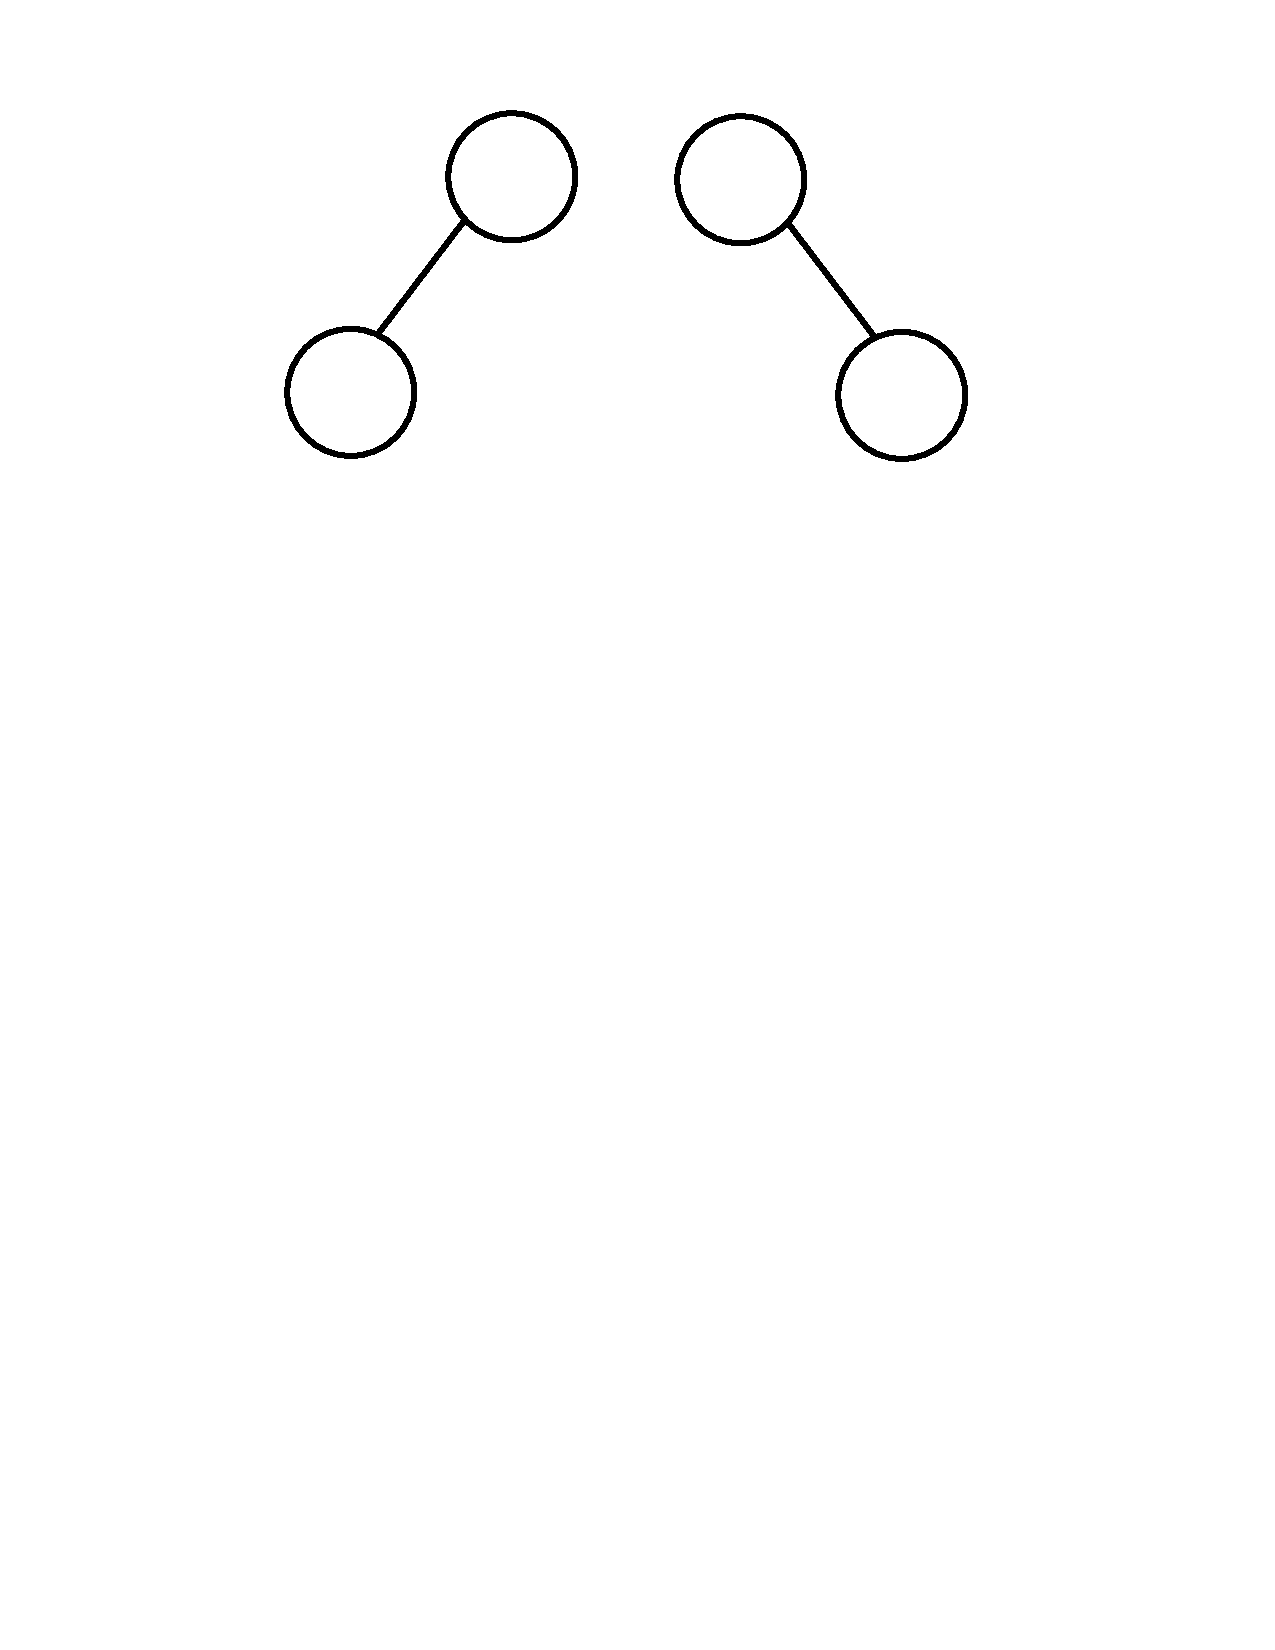
\includegraphics[scale=0.33]{figs/ch5/binary_trees_with_two_nodes.pdf}
\caption{درخت‌های دودویی مختلفی که با دو گره می‌توان ساخت}\label{ch5:fig:2nodesBinTrees}
\end{center}
\end{figure}

\پاسخ

فرض کنید دارای {$n$} گره هستیم که آنها را از 1 تا {$n$} شماره‌گذاری کرده‌ایم و این گره‌ها را به صورت زیر در کنار هم قرار داده‌ایم:
$$
1,2,3,\cdots ,n
$$
با در نظر گرفتن این شماره‌گذاری، مجدداً فرض کنید که گره شماره‌ی {$i$} ({$1\leqslant i \leqslant n$}) ریشه‌ی یک درخت دودویی باشد و تمام گره‌های با شماره کمتر از {$i$} در زیردرخت چپ {$i$} و تمام گره‌های با شماره بیشتر از {$i$} در زیردرخت راست {$i$} قرار بگیرند. در این‌صورت زیردرخت چپ ریشه دارای {$i-1$} گره و  زیردرخت راست دارای {$n-i$} گره خواهند بود.

\begin{figure}
\begin{center}
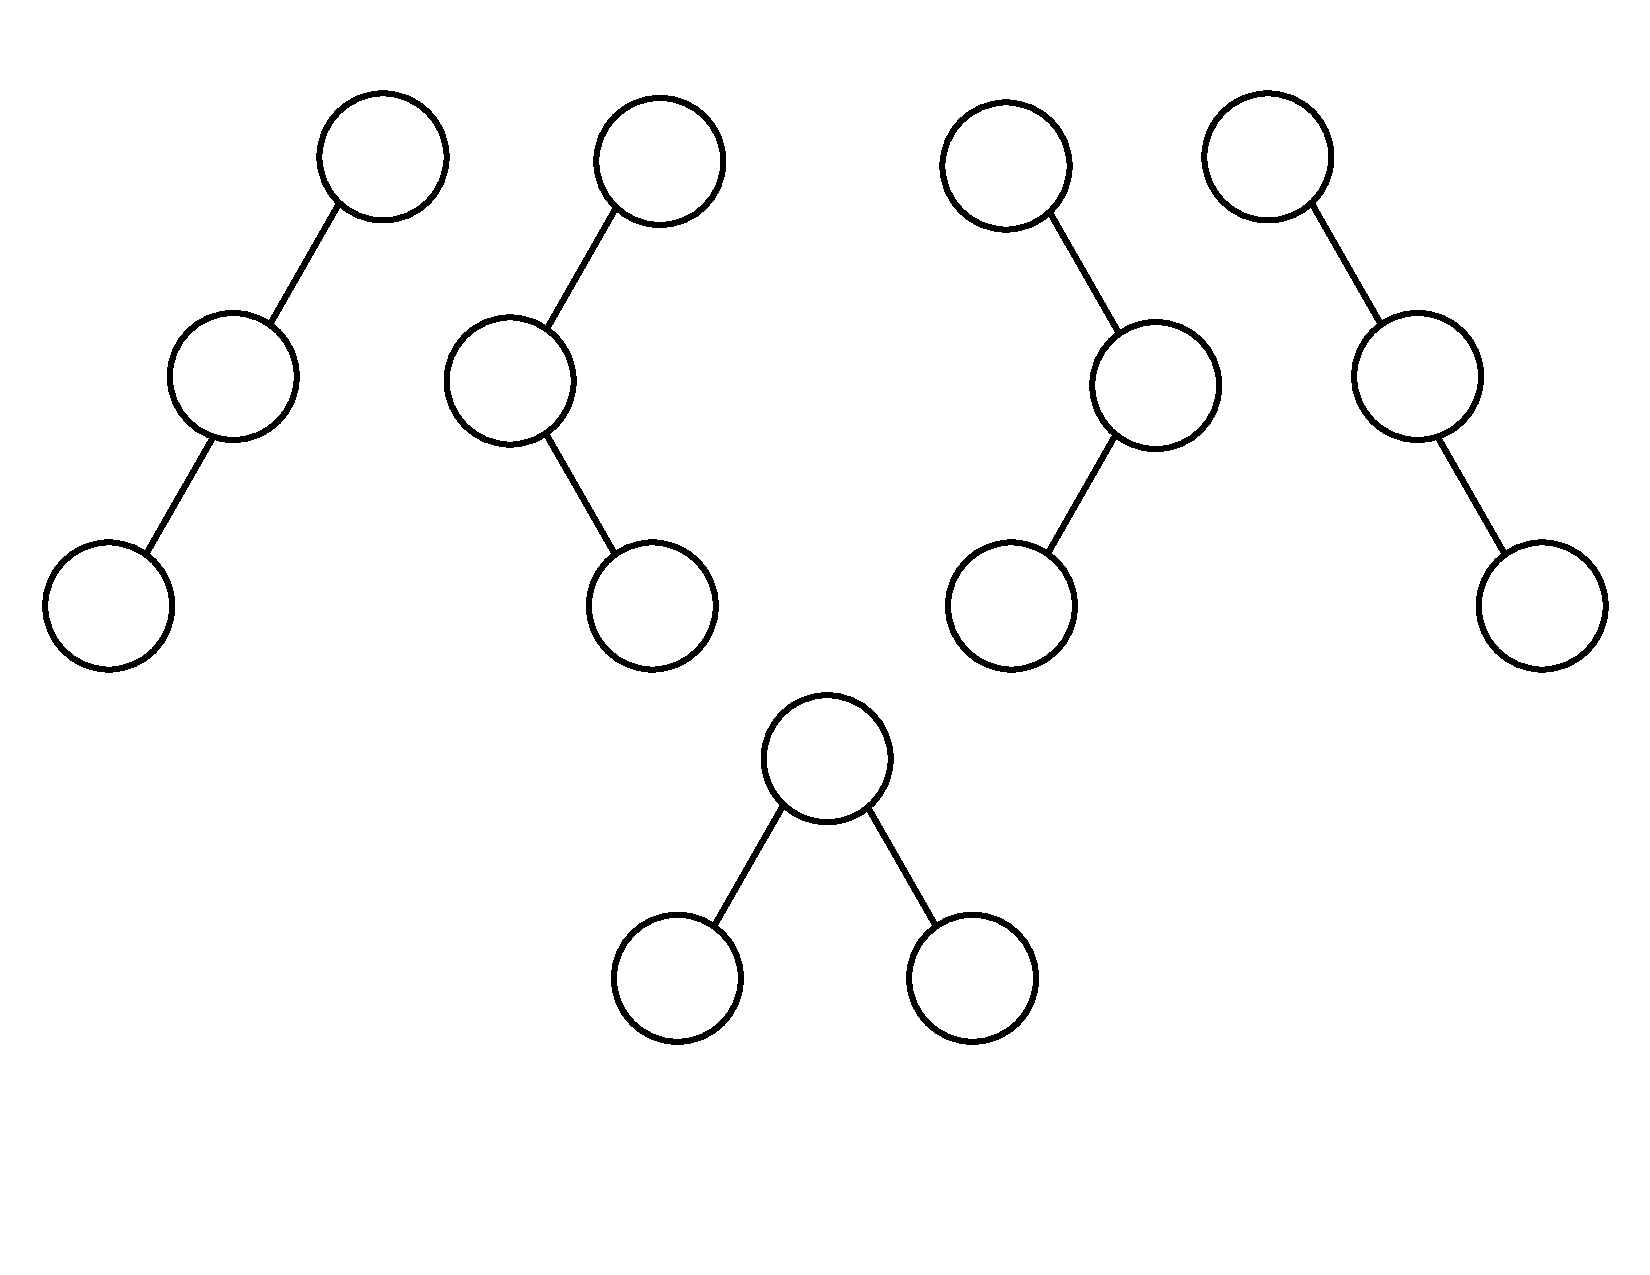
\includegraphics[scale=0.33]{figs/ch5/binary_trees_with_three_nodes.pdf}
\caption{درخت‌های دودویی مختلفی که با سه گره می‌توان ساخت}\label{ch5:fig:3nodesBinTrees}
\end{center}
\end{figure}

 اگر {$T(n)$} را برابر با تعداد درختهای دودویی مختلفی که با {$n$} گره می‌توان ساخت در نظر بگیریم آنگاه تعداد زیردرخت‌های چپ و راست درخت با ریشه {$i$} به ترتیب برابر با {$T(i-1)$} و {$T(n-i)$} خواهند بود. با توجه به اصل شماره دو شمارش، یعنی اصل ضرب، حاصل عبارت {$T(i-1)\cdot T(n-i)$} برابر با تعداد کل درخت‌های دودویی ممکن با ریشه {$i$} است. {$i$} می‌تواند هر یک از مقادیر 1 تا {$n$} را اختیار کند. در نتیجه به ‌منظور در نظر گرفتن کلیه‌ی حالات گره‌ی ریشه، باید  مقدار عبارت {$T(i-1)\cdot T(n-i)$} را برای همه‌ی مقادیر {$i$} با یکدیگر جمع کنیم. بدین ترتیب به رابطه بازگشتی {\eqref{ch5:eqn:catalanRec}} می‌رسیم.
 \begin{equation}
 T(n)=
 \begin{cases}
 T(0)=T(1)=1 & i=0,1\\
 \sum\limits_{i=1}^{n}{T(i-1)\cdot T(n-i)}& i > 1
 \end{cases}\label{ch5:eqn:catalanRec}
 \end{equation}
با حل رابطه‌ی بازگشتی {\eqref{ch5:eqn:catalanRec}} به رابطه‌ی  {\eqref{ch5:eqn:catalanNonRec}} می‌رسیم.
 \begin{equation}
T(n)=\frac{\displaystyle\binom{2n}{n}}{n+1}\label{ch5:eqn:catalanNonRec}
 \end{equation}
به این ترتیب و با استفاده از رابطه‌ی {\eqref{ch5:eqn:catalanNonRec}} می‌توان تعداد درخت‌های دودویی مختلفی که با {$n$} گره می‌توان ساخت را به دست آورد. برای مثال تعداد درخت‌های دودویی مختلفی که با ۳ گره می‌توان ساخت برابر است با:
\begin{displaymath}
T(3)=\frac{\displaystyle\binom{6}{3}}{4}=\frac{20}{4}=5
\end{displaymath}
این درخت‌ها در شکل {\eqref{ch5:fig:3nodesBinTrees}} نشان داده شده‌اند. به دنباله‌ی اعداد حاصل از رابطه‌ی {\eqref{ch5:eqn:catalanNonRec}}، دنباله اعداد کاتالان گفته می‌شود.

 
\سوال درختی دودویی را در نظر بگیرید که به روش فرزند چپ - همنیای راست از یک درخت عمومی به دست آمده است. تابعی بازگشتی بنویسید که چنین درخت دودویی را دریافت کرده و به عنوان خروجی، درخت عمومی معادل با درخت دودویی را بازگرداند.
 
 تابعی بازگشتی بنویسید که با دریافت درخت دودوییِ معادلِ یک درخت عمومی، درخت عمومی را بازسازی کند. تنها ورودی تابع شما باید اشاره‌گر به ریشه درخت دودویی باشد.

\پاسخ

شبه کد تابع تبدیل یک درخت دودویی به درخت عمومی معادل‌ در الگوریتم {\eqref{ch5:alg:cnvBin2Gen}} نشان داده شده است. 
\begin{algorithm}
\caption{تبدیل درخت دودویی به درخت عمومی معادل}\label{ch5:alg:cnvBin2Gen}
\begin{latin}
\begin{algorithmic}[1]
\Function{BinToGen}{$\id{binTree}$}
		\If{$\id{binTree} \isequal \const{null}$}
				\State	\Return \const{null}
		\EndIf
		\State	\bcall{New}{$t$}
		\State	$\attrib{t}{tag} \gets \const{true}$
		\State	$\attrib{t}{data} \gets \attrib{\id{binTree}}{data}$
		\State	$\attrib{t}{link} \gets \const{null}$
		\State	$q \gets t$
		\State	$p \gets \attrib{\id{binTree}}{\id{leftChild}}$
		\While{$p \neq \const{null}$}
				\State	\bcall{New}{$\attrib{q}{\id{link}}$}
				\State	$q \gets \attrib{q}{link}$
				\State	$\attrib{q}{tag} \gets \const{false}$
				\State	$\attrib{q}{dlink} \gets \Call{BinToGen}{p}$
				\State	$\attrib{q}{link} \gets \const{null}$
				\State	$p \gets \attrib{p}{rightChild}$
		\EndWhile
		\State	\Return $t$
\EndFunction
\end{algorithmic}
\end{latin}
\end{algorithm}

\سوال تابعی بازگشتی بنویسید که اشاره‌گر به ریشه‌ی یک درخت دودویی را دریافت کرده و تعداد سطوح آن را بازگرداند.

\پاسخ

شبه کد الگوریتم یافتن تعداد سطوح یک درخت دودویی در الگوریتم {\eqref{ch5:alg:treeLevel}} نشان داده شده است. اگر درخت دودویی ورودی تهی باشد مقدار صفر به عنوان تعداد سطوح درخت بازگردانده می‌شود. در غیر این صورت به صورت بازگشتی به ترتیب تعداد سطوح زیردرخت چپ و راست ریشه به دست آورده می‌شود. سپس تعداد سطوح زیردرخت چپ و راست با یکدیگر مقایسه شده و مقدار بزرگتر با عدد یک جمع شده و در متغیر {\id{level}} قرار می‌گیرد. دلیل جمع شدن مقدار بزرگتر با عدد یک این است که با انجام دو فراخوانی‌ بازگشتی تعداد سطوح دو زیردرخت ریشه را به دست آورده‌ایم و با در نظر گرفتن گره ریشه باید یک واحد به تعداد سطوح درخت اضافه شود. در نهایت متغیر {\id{level}} که بیانگر تعداد سطوح درخت است به عنوان خروجی الگوریتم برگشت داده می‌شود.  

\begin{algorithm}
\caption{به دست آوردن تعداد سطوح یک درخت دودویی}\label{ch5:alg:treeLevel}
\begin{latin}
\begin{algorithmic}[1]
\Function{TreeLevel}{$t$}
		\If{$t \isequal \const{null}$}
			\State	\Return 0
		\EndIf
		\State	$\id{leftLevel} \gets \bcall{TreeLevel}{\attrib{t}{\id{leftChild}}}$
		\State	$\id{rightLevel} \gets \bcall{TreeLevel}{\attrib{t}{\id{rightChild}}}$			
		\If{$\id{leftLevel} > \id{rightLevel}$}
			\State	$\id{level}\gets\id{leftLevel} + 1$
		\Else
			\State	$\id{level}\gets\id{rightLevel} + 1$
		\EndIf
		\State	\Return	\id{level}
\EndFunction
\end{algorithmic}
\end{latin}
\end{algorithm}

\سوال پهنای یک درخت برابر است با تعداد گره‌های سطحی که دارای بیشترین تعداد گره در میان تمام سطوح درخت است.  برای مثال درخت نشان داده شده در شکل {\eqref{ch5:fig:treeWidth}} دارای پهنای چهار است زیرا سطح اول دارای یک گره، سطح دوم دارای دو گره، سطح سوم دارای چهار گره و سطح چهارم دارای یک گره است و در نتیجه حداکثر تعداد گره در یک سطح از این درخت برابر با چهار است و این یعنی پهنای درخت نیز برابر با چهار است. تابعی بازگشتی بنویسید که اشاره‌گر به ریشه‌ی یک درخت دودویی را به عنوان ورودی دریافت کرده و پهنای درخت را به عنوان خروجی بازگرداند (فرض کنید درخت ورودی تهی نیست).

\begin{figure}
\begin{center}
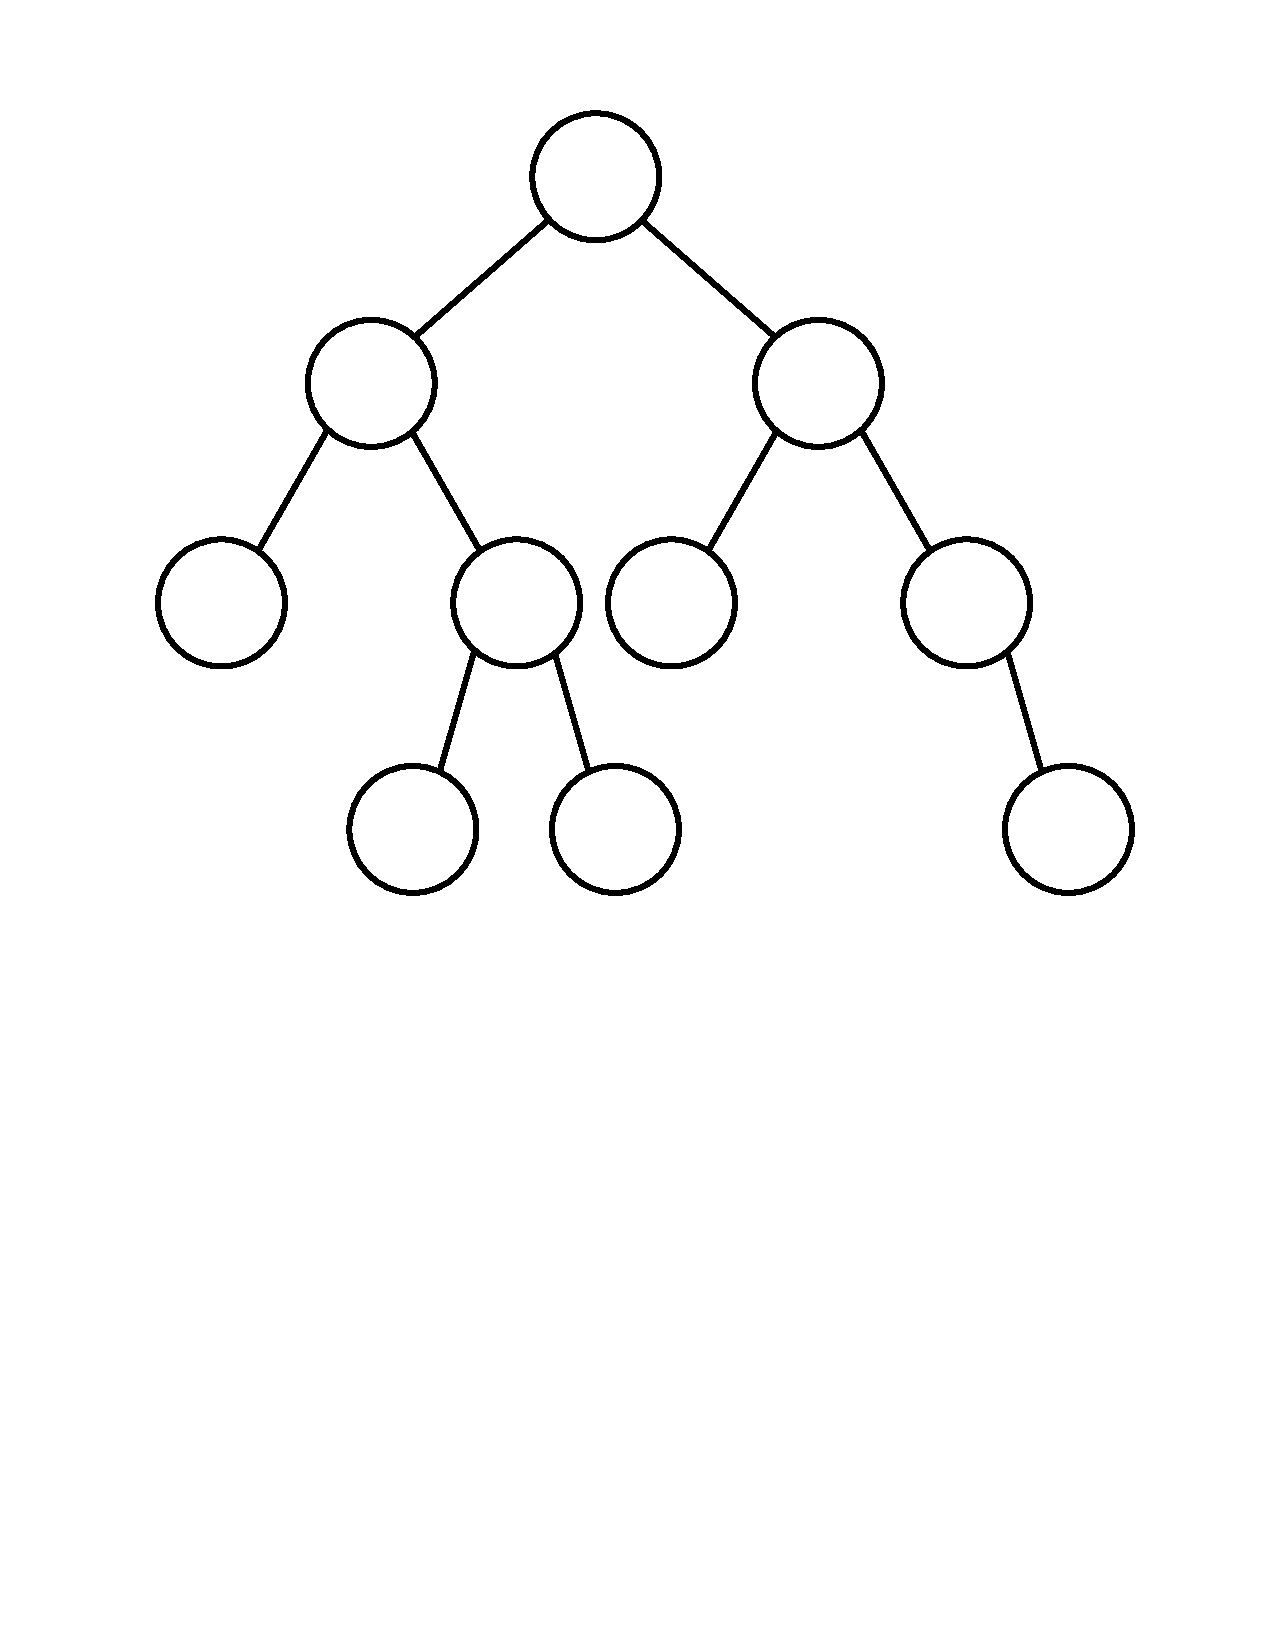
\includegraphics[scale=0.33]{figs/ch5/tree_width.pdf}
\end{center}\caption{درخت دودویی با پهنای چهار}\label{ch5:fig:treeWidth}
\end{figure}

\پاسخ

شبه کد تابع به دست آوردن پهنای یک درخت دودویی در الگوریتم {\eqref{ch5:alg:treeWidth}} نشان داده شده است. این تابع علاوه بر پهنای درخت، شماره سطحی را که تعیین کننده پهنای درخت هست نیز برمی‌گرداند. برای به دست آوردن پهنای درختی دودویی که {$T$} به ریشه آن اشاره دارد تابع {\bcall{TreeWidth}{}} باید به صورت {\bcall{TreeWidth}{$T,1$}} فراخوانی شود. روش کار این تابع در ادامه بیان می‌شود.

زمانی که درخت ورودی تهی است مقدار صفر هم برای سطح و هم برای پهنای درخت بازگردانده می‌شود. اگر درخت ورودی دارای تنها یک عنصر باشد، که همان عنصر ریشه است، مقدار یک هم برای سطح و هم برای پهنای درخت بازگردانده می‌شود و این یعنی درخت دارای پهنای یک است و همچنین سطحی که دارای این پهنا است سطح شماره یک است. زمانی که درخت ورودی دارای بیش از یک عنصر است از فراخوانی بازگشتی استفاده می‌کنیم تا پهنای زیردرخت چپ و راست گره ریشه را به دست بیاوریم. چون پهنای زیر درخت چپ و راست گره ریشه به صورت جداگانه محاسبه می‌شوند باید بررسی کنیم تا در صورتی که {\id{leftLevel}} برابر با {\id{rightLevel}} باشد، مقادیر {\id{leftWidth}} و {\id{rightWidth}} با یکدیگر جمع شوند تا پهنای کلی درخت به دست آید. در صورتی که {\id{leftLevel}} برابر با {\id{rightLevel}} نباشد آنگاه مقدار بزرگتر از میان دو مقدار {\id{leftWidth}} و {\id{rightWidth}} به عنوان پهنای درخت و سطح متناظر با مقدار بزرگتر به عنوان سطحی که تعیین کننده پهنای درخت است به عنوان خروجی تابع بازگردانده می‌شوند.

\begin{algorithm}
\caption{به دست آوردن پهنای یک درخت دودویی}\label{ch5:alg:treeWidth}
\begin{latin}
\begin{algorithmic}[1]
\Function{TreeWidth}{$T,\id{currentLevel}$}
		\If{$\attrib{T}{leftChild} \isequal \const{null} \And \attrib{T}{rightChild} \isequal \const{null}$}
			\State	\Return $(1,\id{currentLevel})$
		\EndIf
		\State	$\id{leftWidth},\id{leftLevel} \gets \bcall{TreeWidth}{\attrib{T}{leftChild},\id{currentLevel}+1}$
		\State	$\id{rightWidth},\id{rightLevel} \gets \bcall{TreeWidth}{\attrib{T}{rightChild},\id{currentLevel}+1}$
		\If{$\id{leftLevel} \isequal \id{rightLevel}$}
			\State	$\id{width} \gets \id{leftWidth}+\id{rightWidth}$
			\State	$\id{level} \gets \id{leftLevel}$
		\Else
			\State	$\id{width} \gets \bcall{Max}{\id{leftWidth},\id{rightWidth}}$
			\If{$\id{leftWidth} > \id{rightWidth}$}
				\State	$\id{width} \gets \id{leftWidth}$
				\State	$\id{level} \gets \id{leftLevel}$
			\Else			
				\State	$\id{width} \gets \id{rightWidth}$			
				\State	$\id{level} \gets \id{rightLevel}$
			\EndIf
		\EndIf
		\State	\Return	$(\id{width},\id{level})$
\EndFunction
\end{algorithmic}
\end{latin}
\end{algorithm}


\سوال ساده‌ترین الگوریتم برای یافتن دومین بزرگترین مقدار در یک آرایه‌ی {$n$} خانه‌ای نیاز به تقریباً {$2n$} مقایسه دارد. گام‌های کلی الگوریتمی را شرح دهید که دومین بزرگترین مقدار در یک آرایه را با حداکثر {$n+2\lfloor \lg n \rfloor - 2$} مقایسه پیدا می‌کند (راهنمایی: فرض کنید تعداد عناصر آرایه زوج است و از درخت‌ برنده-بازنده\پانویس{{\lr{winner-loser tree}}} استفاده کنید).

\پاسخ

این الگوریتم دارای دو مرحله است و در هر مرحله درختی دودویی با نام درخت برنده-بازنده ساخته می‌شود.

در یک درخت برنده-بازنده تمامی عناصر آرایه ورودی به عنوان برگ‌های درخت قرار می‌گیرند. اگر فرض کنیم آرایه ورودی دارای هشت خانه است و حاوی اعداد ۱۹، ۱۳، ۶، ۵، ۳، ۱، ۱۲، ۱۰ است آنگاه درخت برنده-بازنده‌ی ابتدایی در مرحله اول اجرای الگوریتم به صورت شکل {\eqref{ch5:fig:winLose1}} خواهد بود. در هر سطح، عناصری که دارای پدر یکسان هستند با یکدیگر مقایسه شده و مقدار بزرگتر به سطح بالاتر یعنی به گره‌ی پدر آن دو گره‌ای که با یکدیگر مقایسه شده‌اند کپی می‌شود. این روند به همین ترتیب ادامه می‌یابد تا در نهایت گره ریشه بدست آید که همان بزرگترین مقدار آرایه است. درخت نهایی مرحله اول اجرای الگوریتم در شکل {\eqref{ch5:fig:winLose2}} به نمایش در آمده است. 

در این درخت با هر مقایسه‌ای که انجام می‌شود یک برنده، یعنی عنصر با مقدار بزرگتر، و یک بازنده، یعنی عنصر با مقدار کوچکتر، مشخص می‌شوند و مقدار عنصر برنده به سطح بالاتر منتقل می‌شود. با توجه به اینکه هر عنصری غیر از بزرگترین عنصر، دقیقاً یک بار باید بازنده شده‌ باشد می‌توان گفت که تعداد مقایسات لازم برای ساخت چنین درختی برابر با {$n-1$} است. 

\begin{figure}
\begin{center}
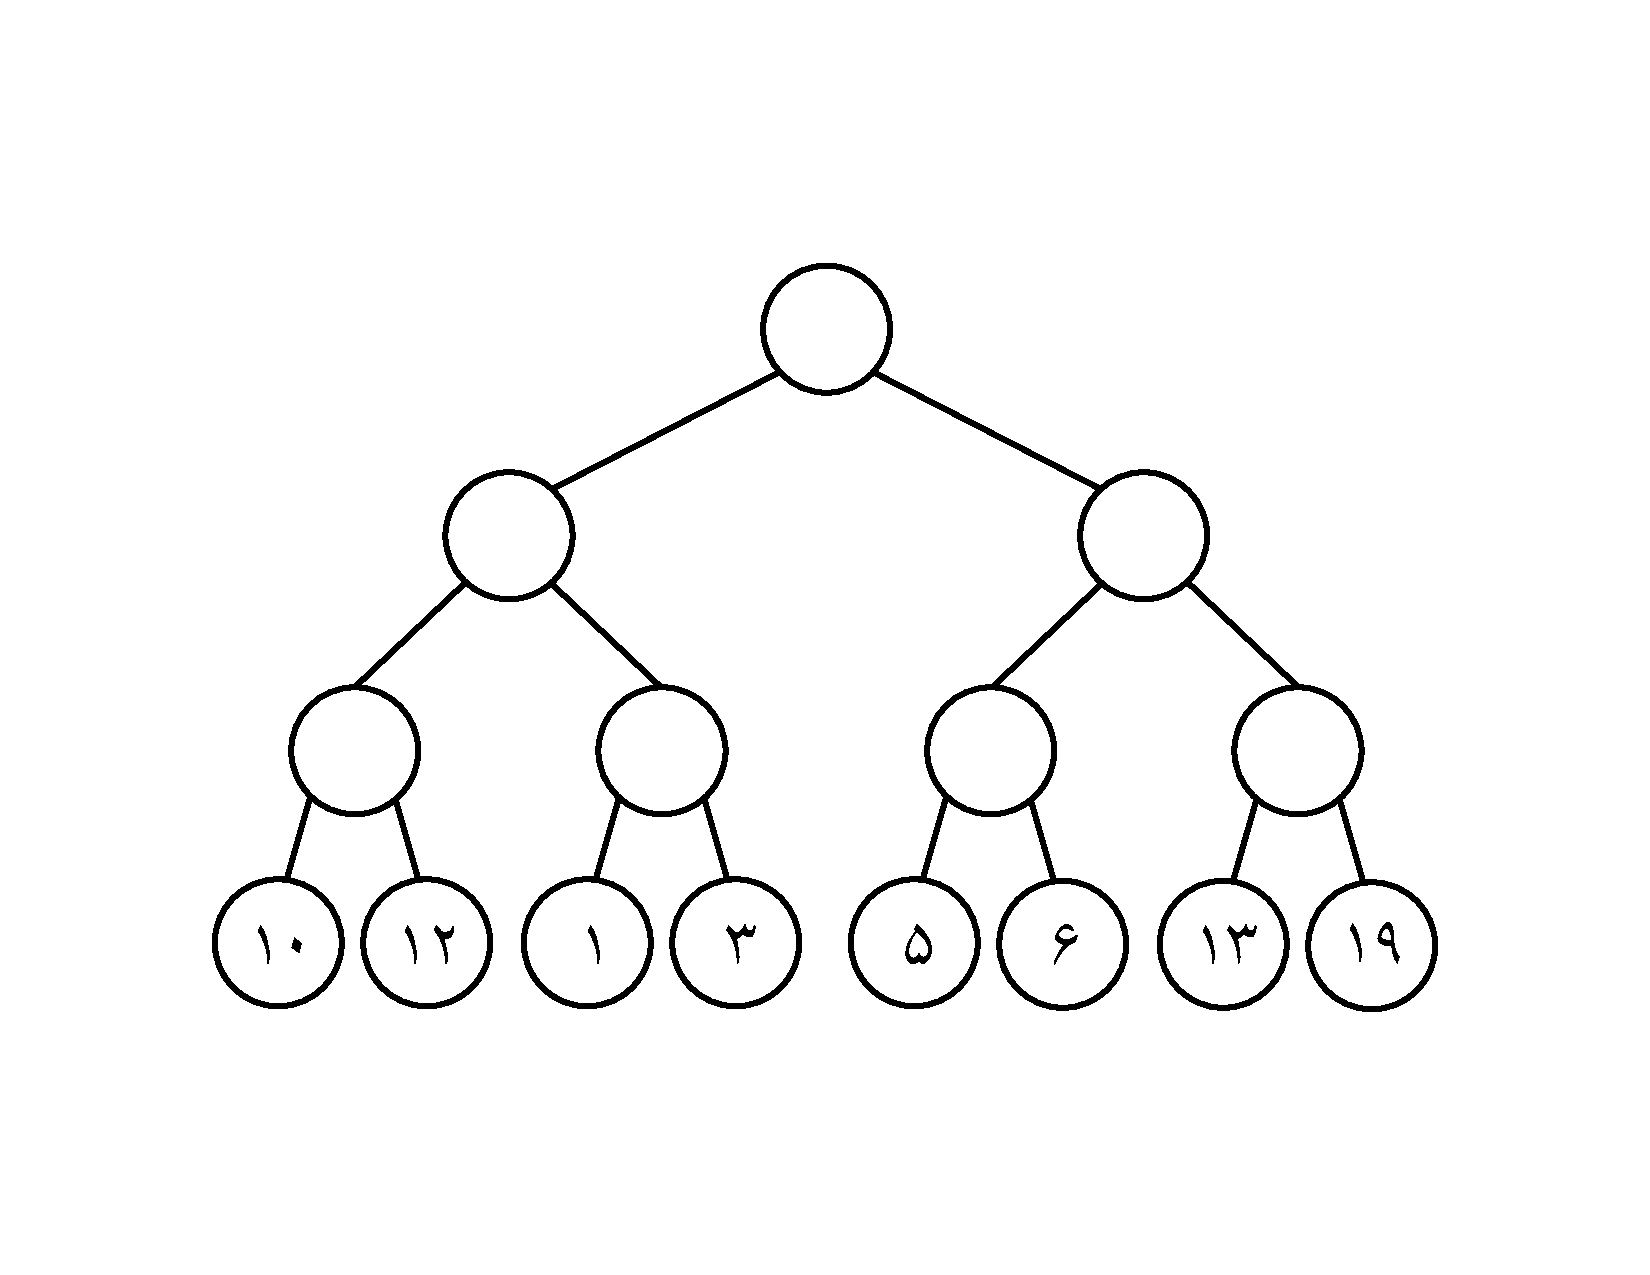
\includegraphics[scale=0.36]{figs/ch5/winner_loser_tree_1.pdf}
\caption{درخت برنده-بازنده در ابتدای مرحله اول از اجرای الگوریتم یافتن دومین بزرگترین مقدار}\label{ch5:fig:winLose1}
\end{center}
\end{figure}

\begin{figure}
\begin{center}
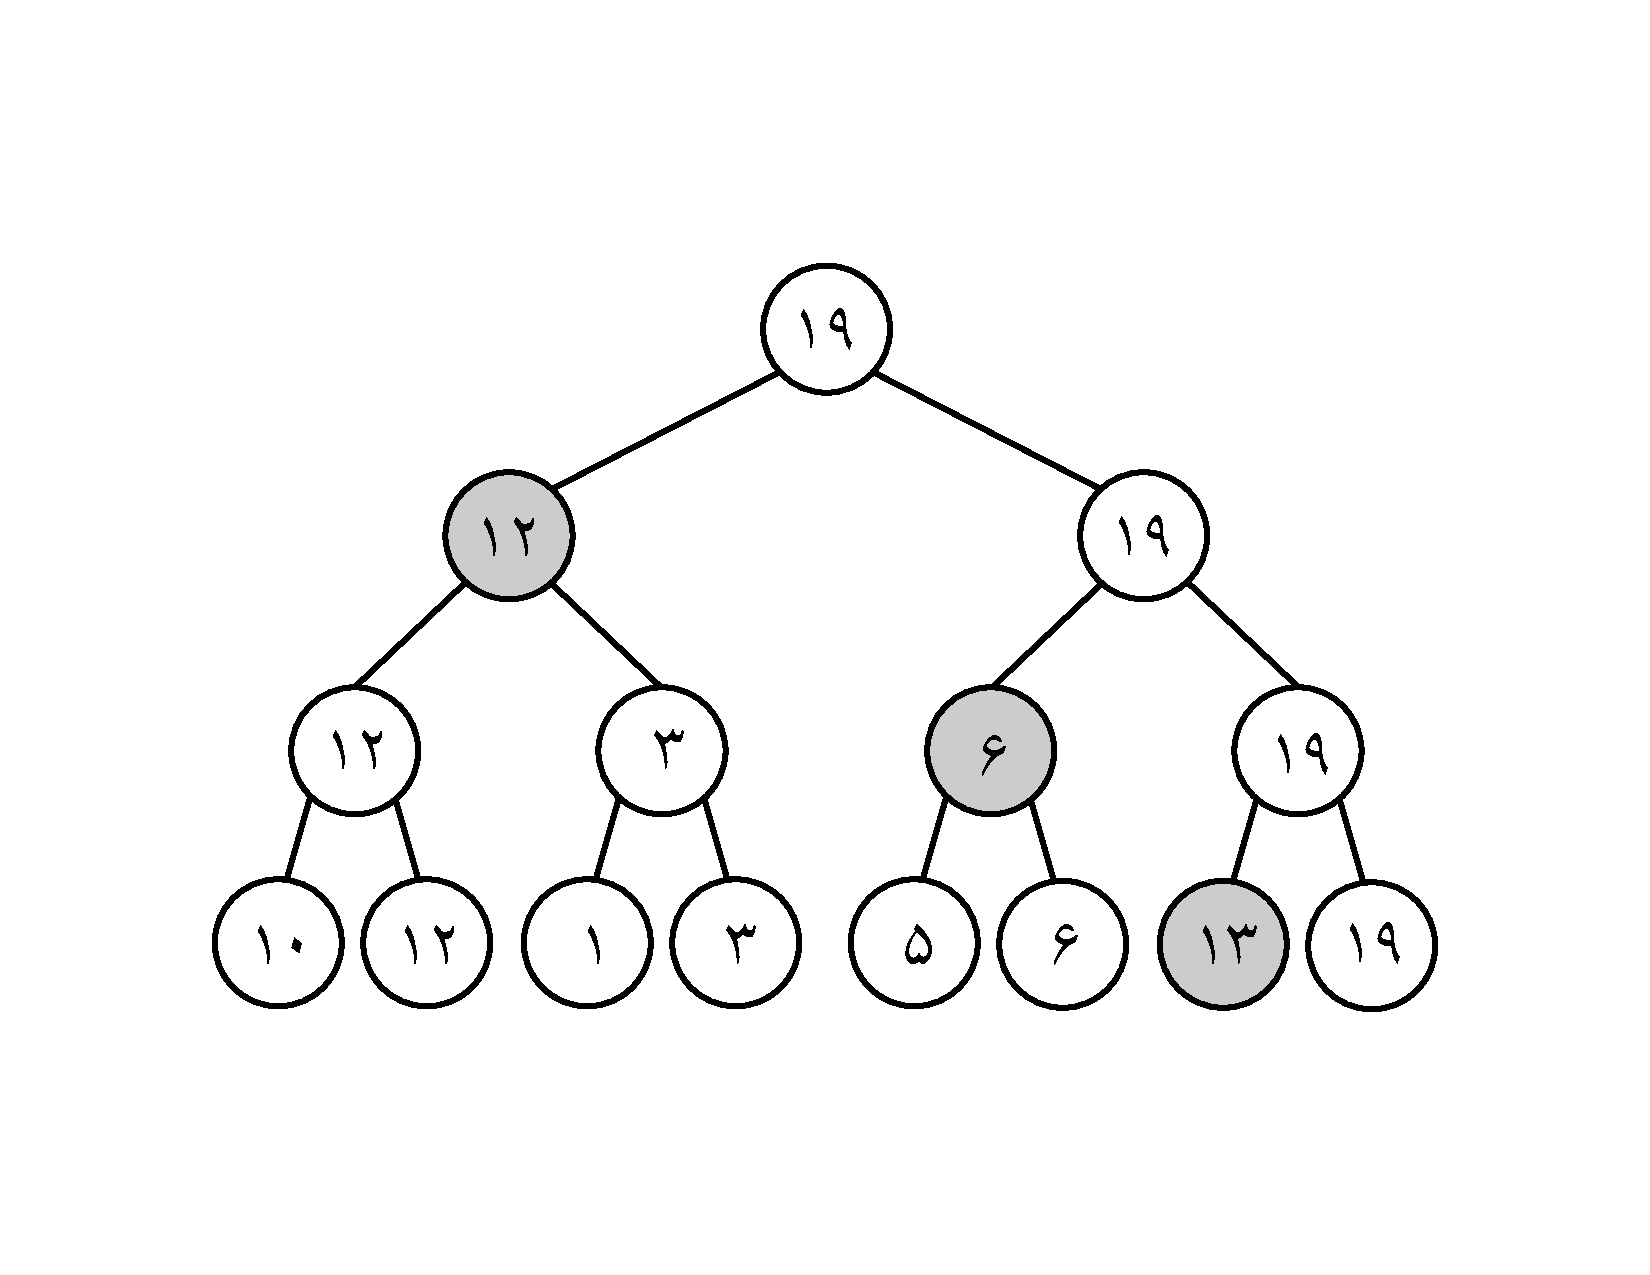
\includegraphics[scale=0.36]{figs/ch5/winner_loser_tree_2.pdf}
\caption{درخت برنده-بازنده در انتهای مرحله اول از اجرای الگوریتم یافتن دومین بزرگترین مقدار}
\label{ch5:fig:winLose2}
\end{center}
\end{figure}

در مرحله دوم اجرای الگوریتم می‌توان گفت عنصر با دومین بزرگترین مقدار، عنصری است که تنها به بزرگترین عنصر، یعنی عنصر ریشه، باخته است. در نتیجه کافی است در مسیر حرکت از گره‌ی ریشه به سمت پایین، در مسیری که بزرگترین عنصر برای رسیدن به گره ریشه طی کرده است حرکت کرده و مقادیری که در مقایسه با گره‌ی ریشه بازنده بوده‌اند را مشخص کنیم (گره‌های خاکستری در شکل  {\eqref{ch5:fig:winLose2}}). 

با توجه به دودویی بودن درخت و تعداد سطوح چنین درختی، تعداد عناصر بازنده به بزرگترین عنصر حداکثر برابر با {$\lfloor\lg n\rfloor$} خواهد بود. لذا {$\lfloor\lg n\rfloor$} مقایسه نیاز خواهیم داشت تا تمام عناصر بازنده به بزرگترین عنصر را به دست بیاوریم. حال برای این
{$\lfloor\lg n\rfloor$} عنصر نیز یک درخت برنده-بازنده می‌سازیم (شکل {\eqref{ch5:fig:winLose3}}) و سپس با {$\lfloor\lg n\rfloor - 1$} مقایسه بزرگترین عنصر این درخت که همان دومین بزرگترین عنصر آرایه است را می‌یابیم. 

به این ترتیب می‌توان گفت حداکثر تعداد مقایسات برای یافتن دومین بزرگترین مقدار در آرایه‌ای {$n$} خانه‌ای برابر با {$n+2\lfloor\lg n\rfloor - 2$} است.

\begin{figure}
\begin{center}
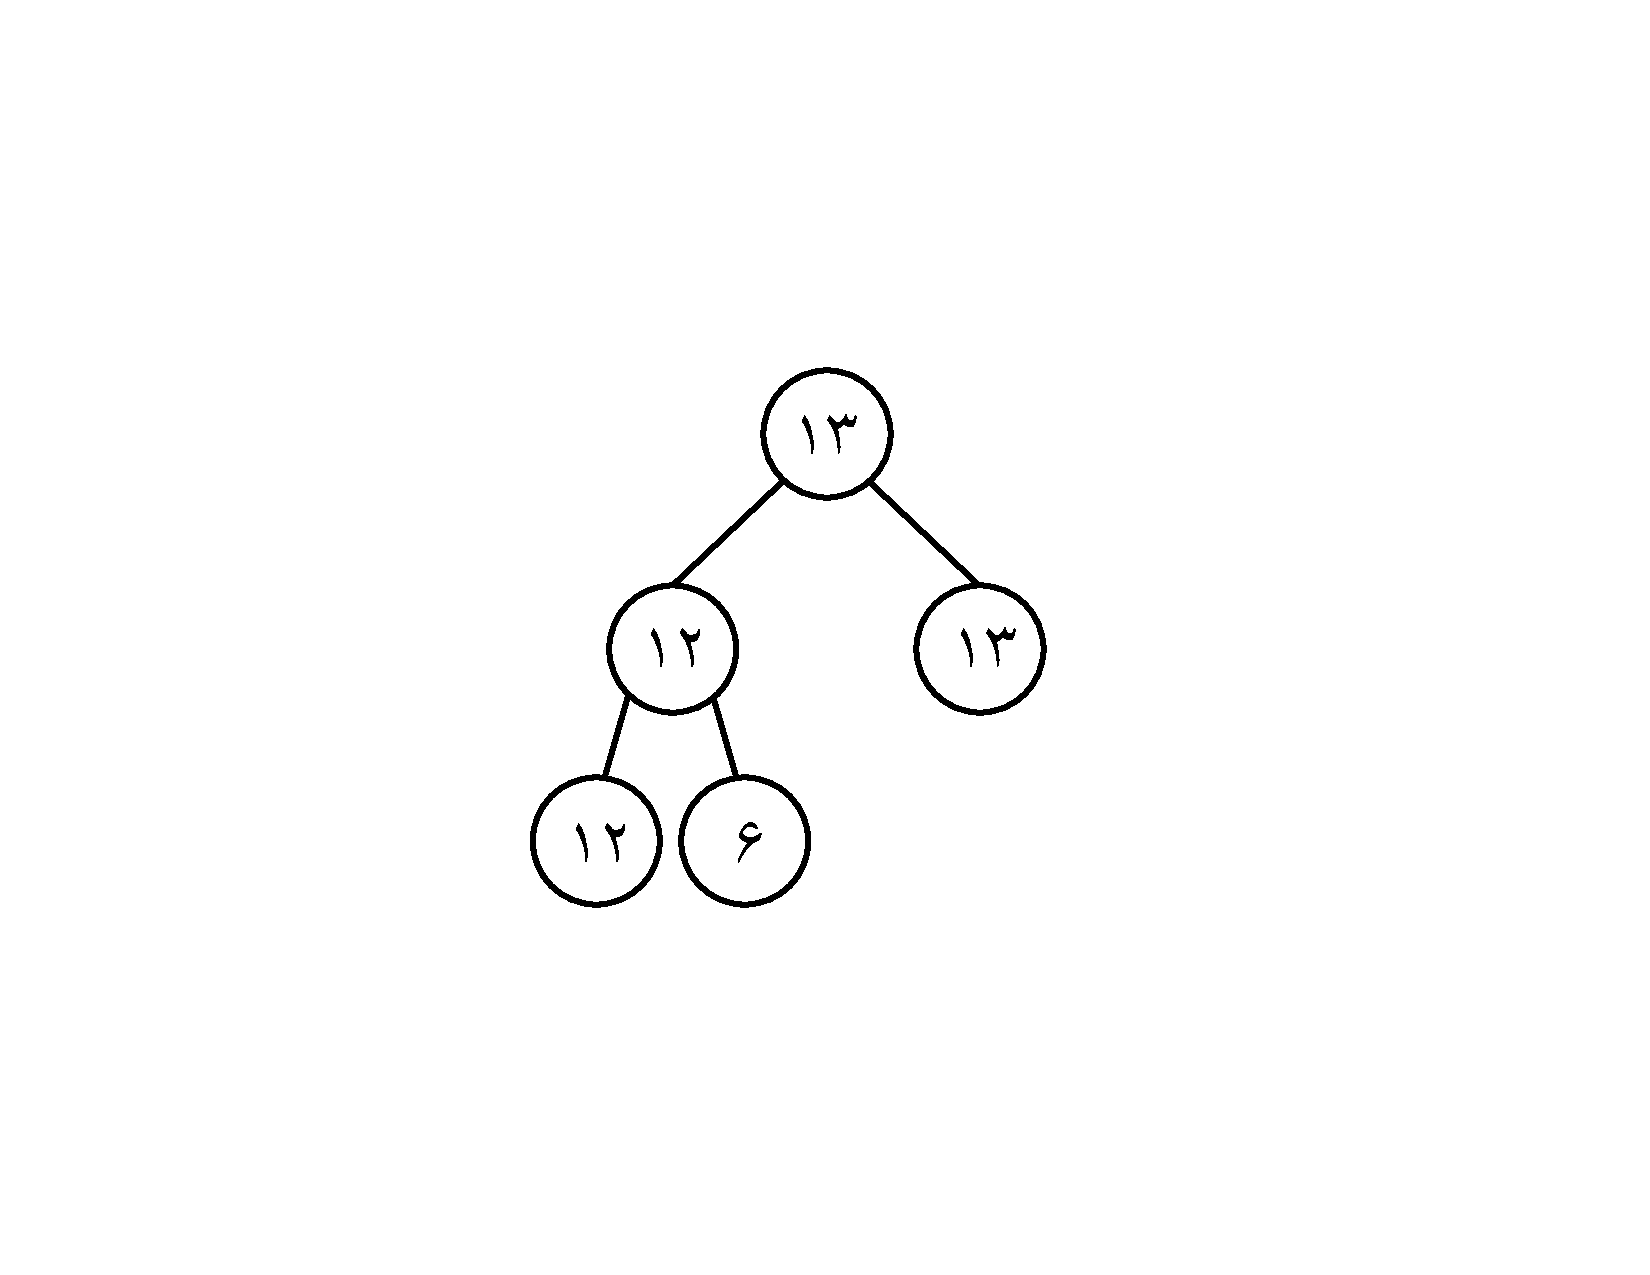
\includegraphics[scale=0.36]{figs/ch5/winner_loser_tree_3.pdf}
\caption{درخت برنده-بازنده در انتهای مرحله دوم از اجرای الگوریم یافتن دومین بزرگترین مقدار}\label{ch5:fig:winLose3}
\end{center}
\end{figure}

\سوال ثابت کنید هر الگوریتم مرتب‌سازی که از مقایسه‌ی عناصر برای تعیین ترتیب صحیح عناصر استفاده می‌کند در بهینه‌ترین حالت از مرتبه {$\Omega (n\lg n)$} است.

\پاسخ

در ابتدا یک مثال ساده را بررسی می‌کنیم. فرض کنید قصد مرتب‌سازی آرایه‌ای سه عنصری را داریم و هر سه عنصر متمایز از یکدیگر هستند. برای نمایش روند مرتب‌سازی عناصر می‌توان از یک درخت دودویی استفاده کرد. در چنین درختی برچسب هر گره نمایش‌دهنده یک مقایسه میان دو عنصر آرایه است و برچسب هر یال نشان دهنده‌ی نتیجه مقایسه دو عنصر است. ترتیب مرتب ‌شده عناصر را می‌توان با حرکت از ریشه‌ی درخت تا یکی از برگ‌ها بدست آورد زیرا هر برگ بیانگر یکی از جایگشت‌های عناصر آرایه است. به چنین درختی، یک درخت تصمیم‌ دودویی\پانویس{{\lr{Binary decision tree}}} گفته می‌شود. شکل {\eqref{ch5:fig:decisionTree}} نشان دهنده‌ی درخت تصمیم دودویی برای یک آرایه سه عنصری است (در این شکل {$x_i$} به معنی مقدار خانه {$i$}ام آرایه است).
\begin{figure}
\begin{center}
\scalebox{0.52}
{
\begin{pspicture}(0,-5.42)(24.52,5.42)
\pscircle[linewidth=0.06,dimen=outer](12.24,4.44){0.98}
\pscircle[linewidth=0.06,dimen=outer](7.48,1.86){0.98}
\pscircle[linewidth=0.06,dimen=outer](16.98,1.88){0.98}
\pscircle[linewidth=0.06,dimen=outer](5.02,-1.32){0.98}
\pscircle[linewidth=0.06,dimen=outer](19.5,-1.28){0.98}
\psellipse[linewidth=0.06,dimen=outer](9.75,-1.34)(2.15,0.8)
\psellipse[linewidth=0.06,dimen=outer](14.51,-1.36)(2.15,0.8)
\psellipse[linewidth=0.06,dimen=outer](2.15,-4.62)(2.15,0.8)
\psellipse[linewidth=0.06,dimen=outer](7.89,-4.6)(2.15,0.8)
\psellipse[linewidth=0.06,dimen=outer](16.63,-4.58)(2.15,0.8)
\psellipse[linewidth=0.06,dimen=outer](22.37,-4.56)(2.15,0.8)
\psline[linewidth=0.04cm](11.52,3.84)(7.44,2.82)
\psline[linewidth=0.04cm](12.98,3.8)(17.02,2.84)
\psline[linewidth=0.04cm](6.88,1.06)(5.04,-0.34)
\psline[linewidth=0.04cm](8.02,1.06)(9.84,-0.52)
\psline[linewidth=0.04cm](16.42,1.06)(14.46,-0.54)
\psline[linewidth=0.04cm](17.56,1.08)(19.5,-0.3)
\psline[linewidth=0.04cm](4.44,-2.14)(2.04,-3.82)
\psline[linewidth=0.04cm](5.58,-2.12)(7.94,-3.78)
\psline[linewidth=0.04cm](18.92,-2.1)(16.52,-3.78)
\psline[linewidth=0.04cm](20.06,-2.08)(22.42,-3.74)
\usefont{T1}{ptm}{m}{it}
\rput(12.244063,4.535){\large\ $x_1 \leq x_2$}
\rput(7.5340624,1.955){\large $x_1 \leq x_3$}
\rput(17.032813,1.975){\large $x_1 \leq x_3$}
\rput(5.098125,-1.265){\large $x_2 \leq x_3$}
\rput(9.7575,-1.34){\Large $\langle x_3,x_1,x_2 \rangle$}
\rput(14.5676565,-1.34){\Large $\langle x_2,x_1,x_3 \rangle$}
\rput(19.574844,-1.31){\large $x_2 \leq x_3$}
\rput(2.1478126,-4.6){\Large $\langle x_1,x_2,x_3 \rangle$}
\rput(7.941875,-4.6){\Large $\langle x_1,x_3,x_2\rangle$}
\rput(16.660625,-4.6){\Large $\langle x_2,x_3,x_1 \rangle$}
\rput(22.376563,-4.6){\Large $\langle x_3,x_2,x_1\rangle$}
\usefont{T1}{ptm}{m}{n}
\rput(9.7775,3.9){\Large \rl{بله}}
\rput(14.941093,3.9){\Large \rl{خیر}}
\rput(5.561875,0.635){\Large \rl{بله}}
\rput(9.471875,0.64){\Large \rl{خیر}}
\rput(15.119687,0.635){\Large \rl{بله}}
\rput(19.489687,0.475){\Large \rl{خیر}}
\rput(2.8504686,-2.645){\Large \rl{بله}}
\rput(7.4204686,-2.645){\Large \rl{خیر}}
\rput(17.281093,-2.645){\Large \rl{بله}}
\rput(21.851093,-2.645){\Large \rl{خیر}}
\end{pspicture}
}\caption{درخت تصمیم دودویی برای مرتب‌سازی سه عنصر}\label{ch5:fig:decisionTree}
\end{center}
\end{figure}

هر الگوریتم مرتب‌سازی مبتنی بر مقایسه، با توجه به مقایساتی که انجام می‌دهد، یک درخت تصمیم دودویی را ایجاد می‌کند. در چنین درختی، طولانی‌ترین مسیر از گره‌ی ریشه به یک گره‌ی برگ بیانگر بدترین حالت ممکن در اجرای الگوریتم است. یعنی در چنین حالتی الگوریتم برای مرتب‌سازی عناصر به بیشترین تعداد مقایسات نیاز دارد. همچنین بهترین حالت در اجرای الگوریتم معادل با کوتاه‌ترین مسیر از گره‌ی ریشه به یک گره‌ی برگ است. حالت متوسط نیز از تقسیم تعداد یال‌های موجود در درخت بر تعداد برگ‌های موجود بدست می‌آید. در حالت متوسط در حقیقت مشخص می‌کنیم  به طور متوسط تعداد یال‌هایی که باید طی شوند تا به یک برگ برسیم چه تعداد است.

اگرچه ممکن است در نگاه اول بتوان با رسم درخت تصمیم دودویی برای هر الگوریتم مرتب‌سازی، به تعیین طول کوتاهترین و طولانی‌ترین مسیر پرداخت امّا حالتی را در نظر بگیرید که قصد مرتب‌سازی آرایه‌ای با ۱۰ عنصر را داریم. درخت تصمیم دودویی چنین آرایه‌ای دارای حداقل {$10!$} برگ است (چون ممکن است برخی از جایگشت‌ها بیش از یکبار ظاهر شوند دارای حداقل این تعداد برگ هستیم) و دارای حداقل ۲۲ سطح است. در نتیجه رسم چنین درختی با این ابعاد منطقی به نظر نمی‌رسد. پس باید دید چگونه می‌توان با استفاده از ایده‌ی درخت تصمیم دودویی به مرتبه زمانی {$\Omega (n\lg n)$} رسید.

باید در حالت کلی بررسی کنیم که حداقل عمق یک درخت تصمیم دودویی برای مرتب‌سازی {$n$} عنصر چه مقداری است. با تعیین این مقدار در حقیقت حداقل تعداد مقایسات در یک الگوریتم مرتب‌سازی مبتنی بر مقایسه را به دست آورده‌ایم.

می‌دانیم که یک درخت تصمیم دودویی برای آرایه‌ای {$n$} عنصری دارای حداقل {$n!$} برگ است. در ادامه حداقل عمق ممکن برای درخت تصمیمی با {$n!$} برگ را محاسبه می‌کنیم. اگر عمق ریشه را برابر با صفر در نظر بگیریم می‌توان گفت در عمق {$k$} تعداد گره‌ها برابر است با {$2^{k}$}. لذا برای داشتن درختی با حداقل {$n!$} برگ، اگر {$k$} را کمترین عمق ممکن برای درخت در نظر بگیریم آنگاه باید داشته باشیم:
\begin{equation}
n!\leq 2^{k}\label{ch5:eqn:dTreeMinDptIneqn1}
\end{equation}
با لگاریتم گرفتن از طرفین نامعادله {\eqref{ch5:eqn:dTreeMinDptIneqn1}} به نامعادله {\eqref{ch5:eqn:dTreeMinDptIneqn2}} می‌رسیم.
\begin{equation}
\lg n! \leq k\label{ch5:eqn:dTreeMinDptIneqn2}
\end{equation}
با درنظر گرفتن این که {$\lg n!$} تقریباً برابر با {$n\lg n -1.5$} است (چرا؟) می‌توان گفت حداقل مقدار {$k$}  تقریباً برابر با {$n\lg n$} است. بدین ترتیب حداقل عمق یک درخت تصمیم دودویی با {$n!$} برگ برابر با {$n\lg n$} است و این یعنی تعداد مقایسات در یک الگوریتم مرتب‌سازی مبتنی بر مقایسه در بهینه‌ترین حالت از مرتبه {$\Omega (n\lg n)$} است. در نتیجه می‌توان گفت هیچ الگوریتم مرتب‌سازی مبتنی بر مقایسه نمی‌تواند در زمانی بهتر از {$\Omega (n\lg n)$} آرایه‌ای {$n$} عنصری را مرتب کند.

\قسمت{درخت‌های هیپ}

\سوال در یک درخت هیپ بیشینه\پانویس{{\lr{Max heap}}} با {$n$} عنصر متمایز، اعمال زیر را با چه مرتبه‌ای می‌توان انجام داد؟ توضیح دهید.
\شروع{فقرات}
\فقره به دست آوردن مجموع همه‌ی اعداد موجود در هیپ
\فقره به دست آوردن مجموع {$\lg n$} بزرگترین اعداد موجود در هیپ
\فقره به دست آوردن مجموع ۱۰ عدد بزرگ موجود در هیپ
\پایان{فقرات}

\پاسخ

برای به دست آوردن مجموع  اعداد موجود در درخت هیپ کافیست درخت را با استفاده از یک پیمایش دلخواه، مثلا میان‌ترتیب، پیمایش کرده و در حین پیمایش با ملاقات هر گره مقدار آن را به مقدار مجموع اضافه کنیم. با توجه به اینکه مرتبه پیمایش میان‌ترتیب برابر با {$O(n)$} است پس مرتبه اجرایی این الگوریتم نیز برابر با {$O(n)$} است.

برای به دست آوردن مجموع {$\lg n$} بزرگترین اعداد موجود در هیپ می‌توان به تعداد {$\lg n$} بار عمل حذف عنصر ریشه را انجام داد و مقدار عدد حذف شده را به مقدار مجموع اضافه کرد. به این ترتیب در بار اول بزرگترین عدد، که در ریشه هیپ است، حذف شده و مقدار آن به مقدار مجموع اضافه می‌شود سپس دومین بزرگترین عنصر حذف شده و به مقدار مجموع اضافه شده و به همین ترتیب. با توجه به اینکه هر عمل حذف از هیپ از مرتبه {$O(\lg n)$} است پس مرتبه کلی الگوریتم برابر خواهد بود با {$\lg n \times O(\lg n)=O({\lg}^2 n)$}.

به دست آوردن مجموع ۱۰ عدد بزرگتر هیپ حالت خاصی از الگوریتم قبلی است. یعنی کافیست ۱۰ بار عنصر ریشه را حذف کرده و هر بار مقدار عنصر حذف شده را به یک متغیر که حاصل جمع را نگه می‌دارد اضافه کنیم. مرتبه زمانی انجام چنین کاری برابر است با {$10\times O(\lg n)=O(\lg n)$}

\سوال در یک درخت هیپ بیشینه حاوی {$n$} عدد متمایز، چهارمین بزرگترین عدد ممکن است در کدامیک از خانه‌های آرایه‌ی حاوی هیپ بیشینه قرار داشته باشد؟‌

\پاسخ

برای تعیین اینکه چهارمین بزرگترین مقدار می‌تواند در کدامیک از خانه‌های آرایه قرار بگیرد باید به طور کلی به دنبال این باشیم که {$k$}امین بزرگترین مقدار در چه سطوحی از درخت هیپ می‌تواند ظاهر شود. سپس شماره‌ی خانه‌های متناظر این سطوح در آرایه را یافته و به این ترتیب بازه‌ای از خانه‌های آرایه که می‌تواند حاوی {$k$}امین بزرگترین مقدار باشد مشخص می‌شود.

بزرگترین مقدار همواره در سطح اول درخت که تنها شامل گره‌ی ریشه است قرار می‌گیرد. دومین بزرگترین مقدار می‌تواند در یکی از دو گره‌ی سطح دوم قرار بگیرد. سومین بزرگترین مقدار می‌تواند در یکی از گره‌های سطوح دوم یا سوم قرار بگیرد. می‌توان اثبات کرد که {$k$}امین بزرگترین مقدار می‌تواند در یکی از سطوح ۲ تا {$k$} قرار بگیرد (طبق آنچه گفته شد برای حالت خاص {$k=1$} این رابطه برقرار نیست و بزرگترین مقدار در سطح یک قرار خواهد گرفت).

بزرگترین مقدار در خانه‌ی شماره یک آرایه قرار می‌گیرد. دومین بزرگترین مقدار می‌تواند در سطح دو (خانه‌های دو یا سه) یا سطح سه (خانه‌های چهار تا هفت) قرار بگیرد (در مجموع خانه‌های دو تا هفت). به همین ترتیب می‌توان گفت {$k$}امین بزرگترین مقدار می‌تواند در یکی از خانه‌های ۲ تا {$2^k-1$} قرار بگیرد.

با توجه به اینکه یک فرمول کلی به دست آوردیم در نتیجه می‌توان گفت چهارمین بزرگترین مقدار می‌تواند در یکی از خانه‌های دو تا پانزده آرایه قرار بگیرد.

\سوال یک درخت هیپ بیشینه شامل اعداد ۱ تا ۱۰۲۳ را در نظر بگیرید. الف) چه تعداد از اعداد بزرگتر از ۱۰۰۰ می‌توانند در گره‌های برگ چنین درختی قرار بگیرند؟ ب) حداکثر چه تعداد از اعداد بزرگتر از ۱۰۰۰ می‌توانند بطور همزمان برگ باشند؟

\پاسخ

برای پاسخ به این سوال به دو نکته‌ی زیر توجه می‌کنیم:
\شروع{شمارش}
\فقره در یک درخت هیپ {$k$}امین بزرگترین عنصر می‌تواند در یکی از سطوح دوم، سوم، {\ldots}، {$k$}ام قرار بگیرد.
\فقره  یک درخت هیپ که حاوی اعداد ۱ تا ۱۰۲۳ است دارای ده سطح است.
\پایان{شمارش}

الف)

با در نظر گرفتن دو نکته‌ی مطرح شده می‌توان گفت عدد ۱۰۲۳ در سطح اول، عدد ۱۰۲۲ در سطح دوم، عدد ۱۰۲۱ در یکی از سطوح دوم یا سوم و به همین ترتیب تا عدد ۱۰۱۵ که در یکی از سطوح دوم تا نهم قرار می‌گیرند. در نتیجه می‌توان گفت اعداد ۱۰۱۵ تا ۱۰۲۳ نمی‌توانند در سطح دهم قرار بگیرند و این یعنی این اعداد نمی‌توانند به عنوان برگ این درخت هیپ بیشینه ظاهر شوند. به بیان دیگر چهارده عدد بزرگتر از ۱۰۰۰ این امکان را دارند که به عنوان برگ درخت هیپ ظاهر شوند و این اعداد عبارتند از ۱۰۰۱ تا ۱۰۱۴.

ب)

برای پاسخ به این قسمت باید طوری اعداد را در هیپ بیشینه قرار دهیم که تا حد ممکن بیشترین اعداد در بازه ۱۰۰۱ تا ۱۰۲۳ در گره‌های برگ ظاهر شوند.

می‌دانیم که بزرگترین مقدار یعنی ۱۰۲۳ در سطح اول، دومین بزرگترین مقدار یعنی ۱۰۲۲ در سطح دوم، سومین بزرگترین مقدار در یکی از سطوح دوم یا سوم و به همین ترتیب ظاهر می‌شوند. حال برای آنکه بیشترین تعداد از اعداد در بازه ۱۰۰۱ تا ۱۰۲۳ در برگ‌ها ظاهر شوند، سعی می‌کنیم اعداد ۱ تا ۵۱۱ را زیردرخت چپ ریشه و اعداد ۵۱۲ تا ۱۰۲۲ را در زیردرخت راست ریشه قرار دهیم (می‌توانستیم به صورت برعکس نیز عمل کنیم بدین معنی که اعداد ۱ تا ۵۱۱ را زیردرخت راست ریشه و اعداد ۵۱۲ تا ۱۰۲۲ را در زیردرخت چپ ریشه قرار دهیم). با توجه به اینکه اعداد مورد نظر ما یعنی ۱۰۰۱ تا ۱۰۲۲ در زیردرخت راست قرار دارند در نتیجه برای ادامه کار فقط به زیردرخت راست توجه می‌کنیم و زیردرخت چپ ریشه را نادیده می‌گیریم. 

در زیردرخت راست، عدد ۱۰۲۲ را به عنوان گره ریشه این زیردرخت در نظر می‌گیریم  و در زیردرخت چپ این گره اعداد ۵۱۲ تا ۷۶۶ و در زیردرخت راست آن اعداد ۷۶۷ تا ۱۰۲۱ را قرار می‌دهیم. مجدداً برای زیردرخت با ریشه ۱۰۲۲ سعی می‌کنیم اعداد ۷۶۷ تا ۸۹۳ را در زیردرخت چپ و اعداد ۸۹۴ تا ۱۰۲۱ را در زیردرخت راست قرار دهیم.  اگر همین روند را ادامه دهیم در سطح ششم درخت به حالتی می‌رسیم که در آن باید اعداد ۹۸۸ تا ۱۰۱۸ را در درخت قرار دهیم. در این حالت نیز به این صورت عمل می‌کنیم که عدد ۱۰۱۸ را در ریشه، اعداد ۹۸۸ تا ۱۰۰۲ را در زیردرخت چپ و اعداد ۱۰۰۳ تا ۱۰۱۷ را در زیردرخت راست قرار می‌دهیم. درخت هیپ مورد نظر تا این مرحله در شکل {\eqref{ch5:fig:maxHeap}} نشان داده شده است.

در این حالت می‌توان گفت زیردرخت حاوی اعداد ۱۰۰۳ تا ۱۰۱۷ دارای چهار سطح است و در نتیجه دارای هشت برگ است. به این ترتیب اعداد ۱۱۶، ۱۱۵ و ۱۱۴ با توجه به اینکه اولین، دومین و سومین بزرگترین مقادیر در این زیردرخت هستند در نتیجه نمی‌توانند در سطح چهارم این زیردرخت (یعنی به عنوان گره‌ی برگ) ظاهر شوند. پس می‌توان گفت در زیردرخت راست گره‌ای که دارای مقدار ۱۰۱۸ در ریشه خود است، هشت عنصر بزرگتر از ۱۰۰۰ و کوچکتر از ۱۰۱۴ می‌توانند به طور همزمان در برگهای درخت هیپ ظاهر شوند. 

در مورد ۱۰۰۱ و ۱۰۰۲ باید گفت با توجه به اینکه ۱۰۰۱ و ۱۰۰۲ در زیردرخت حاوی این اعداد، به ترتیب اولین و دومین بزرگترین عناصر هستند در نتیجه در زیردرخت خود نمی‌توانند به عنوان برگ ظاهر شوند. 
\begin{figure}
\begin{center}
\scalebox{0.7}
{
\begin{pspicture}(0,-6.15)(15.189345,6.11)
\pscircle[linewidth=0.04,dimen=outer](3.08,5.61){0.5}
\usefont{T1}{ptm}{m}{n}
\rput(3.0639062,5.6){$1023$}
\pstriangle[linewidth=0.04,dimen=outer](1.21,3.27)(2.42,1.04)
\pscircle[linewidth=0.04,dimen=outer](4.9,3.81){0.5}
\rput(4.891406,3.8){$1022$}
\psline[linewidth=0.04cm,arrowsize=0.05291667cm 2.0,arrowlength=1.4,arrowinset=0.4]{->}(2.72,5.27)(1.26,4.43)
\psline[linewidth=0.04cm,arrowsize=0.05291667cm 2.0,arrowlength=1.4,arrowinset=0.4]{->}(3.46,5.27)(4.9,4.39)
\pstriangle[linewidth=0.04,dimen=outer](3.01,1.51)(2.42,1.04)
\pscircle[linewidth=0.04,dimen=outer](6.7,2.03){0.5}
\rput(6.676875,2.02){$1021$}
\psline[linewidth=0.04cm,arrowsize=0.05291667cm 2.0,arrowlength=1.4,arrowinset=0.4]{->}(4.52,3.49)(3.06,2.65)
\psline[linewidth=0.04cm,arrowsize=0.05291667cm 2.0,arrowlength=1.4,arrowinset=0.4]{->}(5.26,3.49)(6.7,2.61)
\pstriangle[linewidth=0.04,dimen=outer](4.81,-0.29)(2.42,1.04)
\pscircle[linewidth=0.04,dimen=outer](8.52,0.25){0.5}
\rput(8.5125,0.24){$1020$}
\psline[linewidth=0.04cm,arrowsize=0.05291667cm 2.0,arrowlength=1.4,arrowinset=0.4]{->}(6.34,1.71)(4.88,0.87)
\psline[linewidth=0.04cm,arrowsize=0.05291667cm 2.0,arrowlength=1.4,arrowinset=0.4]{->}(7.08,1.71)(8.52,0.83)
\pstriangle[linewidth=0.04,dimen=outer](6.63,-2.05)(2.42,1.04)
\pscircle[linewidth=0.04,dimen=outer](10.32,-1.53){0.5}
\rput(10.31125,-1.54){$1019$}
\psline[linewidth=0.04cm,arrowsize=0.05291667cm 2.0,arrowlength=1.4,arrowinset=0.4]{->}(8.14,-0.07)(6.68,-0.91)
\psline[linewidth=0.04cm,arrowsize=0.05291667cm 2.0,arrowlength=1.4,arrowinset=0.4]{->}(8.88,-0.07)(10.32,-0.95)
\pstriangle[linewidth=0.04,dimen=outer](8.45,-3.85)(2.42,1.04)
\pscircle[linewidth=0.04,dimen=outer](12.14,-3.33){0.5}
\rput(12.128593,-3.36){$1018$}
\psline[linewidth=0.04cm,arrowsize=0.05291667cm 2.0,arrowlength=1.4,arrowinset=0.4]{->}(9.96,-1.87)(8.5,-2.71)
\psline[linewidth=0.04cm,arrowsize=0.05291667cm 2.0,arrowlength=1.4,arrowinset=0.4]{->}(10.7,-1.87)(12.14,-2.75)
\pstriangle[linewidth=0.04,dimen=outer](10.23,-5.63)(2.42,1.04)
\psline[linewidth=0.04cm,arrowsize=0.05291667cm 2.0,arrowlength=1.4,arrowinset=0.4]{->}(11.78,-3.65)(10.32,-4.49)
\psline[linewidth=0.04cm,arrowsize=0.05291667cm 2.0,arrowlength=1.4,arrowinset=0.4]{->}(12.52,-3.65)(13.96,-4.53)
\pstriangle[linewidth=0.04,dimen=outer](14.01,-5.63)(2.42,1.04)
\usefont{T1}{ptm}{m}{n}
\rput(1.166875,2.98){$1,\ldots,511$}
\usefont{T1}{ptm}{m}{n}
\rput(2.9945312,1.18){$512,\ldots,766$}
\usefont{T1}{ptm}{m}{n}
\rput(4.8082814,-0.64){$767,\ldots,893$}
\usefont{T1}{ptm}{m}{n}
\rput(6.6121874,-2.38){$894,\ldots,956$}
\usefont{T1}{ptm}{m}{n}
\rput(8.434844,-4.16){$957,\ldots,987$}
\usefont{T1}{ptm}{m}{n}
\rput(10.185312,-5.94){$988,\ldots,1002$}
\usefont{T1}{ptm}{m}{n}
\rput(14.000937,-5.92){$1003,\ldots,1017$}
\end{pspicture} 
}\caption{درخت هیپ بیشینه حاوی اعداد ۱ تا ۱۰۲۳}\label{ch5:fig:maxHeap}
\end{center}
\end{figure}

به عنوان نتیجه‌گیری می‌توان گفت اعداد ۱۰۰۱ تا ۱۰۱۴ این امکان را دارند که به عنوان گره‌ی برگ در درخت هیپ بیشینه ظاهر شوند اما فقط هشت عدد از میان اعداد ۱۰۰۳ تا ۱۰۱۳ این امکان را دارند که بطور همزمان در گره‌های برگ ظاهر شوند.

\سوال داده‌ساختار صف اولویت میانه\پانویس{{\lr{Median priority queue}}}، یک داده‌ساختار شامل {$n$} عنصر با مقادیر متمایز است که می‌توان اعمال زیر را بر روی آن انجام داد:
\شروع{فقرات}
\فقره درج یک عنصر در زمان {$O(\lg n)$}
\فقره حذف عنصر دارای مقدار میانه در زمان {$O(\lg n)$}
\پایان{فقرات}
با استفاده از داده‌ساختار درخت هیپ، داده‌ساختار صف اولویت میانه را طراحی کنید. سپس نحوه‌ی انجام اعمال نامبرده با پیچیدگی زمانی خواسته شده را شرح دهید.

\پاسخ

عنصر میانه در یک لیست، عنصری است که از نیمی از داده‌های لیست بزرگتر و از نیمی از داده‌ها کوچکتر است. از همین ویژگی برای طراحی داده‌ساختار صف اولویت میانه استفاده خواهیم کرد.

در لیستی با تعداد عناصر فرد، عنصر میانه عنصری است که پس از مرتب کردن عناصر لیست در وسط لیست قرار می‌گیرد. به طور مثال لیست {$L=\langle 4,2,3,5,1 \rangle$} را در نظر بگیرید. پس از مرتب کردن عناصر لیست {$L$}، به لیست {$L=\langle 1,2,3,4,5 \rangle$} می‌رسیم. بدین ترتیب میانه‌ لیست {$L$} عدد ۳ خواهد بود. به عبارت بهتر اگر در لیستی با تعداد عناصر فرد تعداد عناصر را با {$n$} نشان دهیم  عنصر میانه پس از مرتب‌سازی لیست در مکان {$\lfloor n/2 \rfloor +1$} قرار خواهد گرفت. در لیستی {$n$} عنصری با زوج عنصر، با توجه به اینکه دارای عنصر وسط نیستیم، می‌توان پس از مرتب کردن لیست، عنصر موجود در مکان {$\lfloor n/2 \rfloor$} یا {$\lfloor n/2 \rfloor +1$} را به عنوان عنصر میانه در نظر گرفت. 

فرض کنید می‌خواهیم عنصر میانه را از لیست {$L=\langle 4,2,3,5,1 \rangle$} حذف کنیم. در این صورت باید عدد ۲ (بزرگترین عددی که کوچکتر از میانه است) یا ۴ (کوچکترین عددی که از میانه بزرگتر است) را به عنوان عنصر میانه‌ی جدید برگزینیم. برای این منظور می‌توان درختی دودویی را در نظر گرفت که در آن زیردرخت چپ ریشه یک درخت هیپ بیشینه و زیردرخت راست ریشه یک درخت هیپ کمینه است. عناصر کمتر از میانه‌ی جاری را در هیپ بیشینه و عناصر بیشتر از میانه‌ی جاری را در هیپ کمینه نگه می‌داریم. شکل این روش ذخیره‌سازی داده‌ساختار صف اولویت میانه برای لیستی مانند {$L=\langle 4,2,3,5,1 \rangle$} به صورت نشان داده شده در شکل {\eqref{ch5:fig:medPrioQueue1}} خواهد بود.

\begin{figure}
\begin{center}
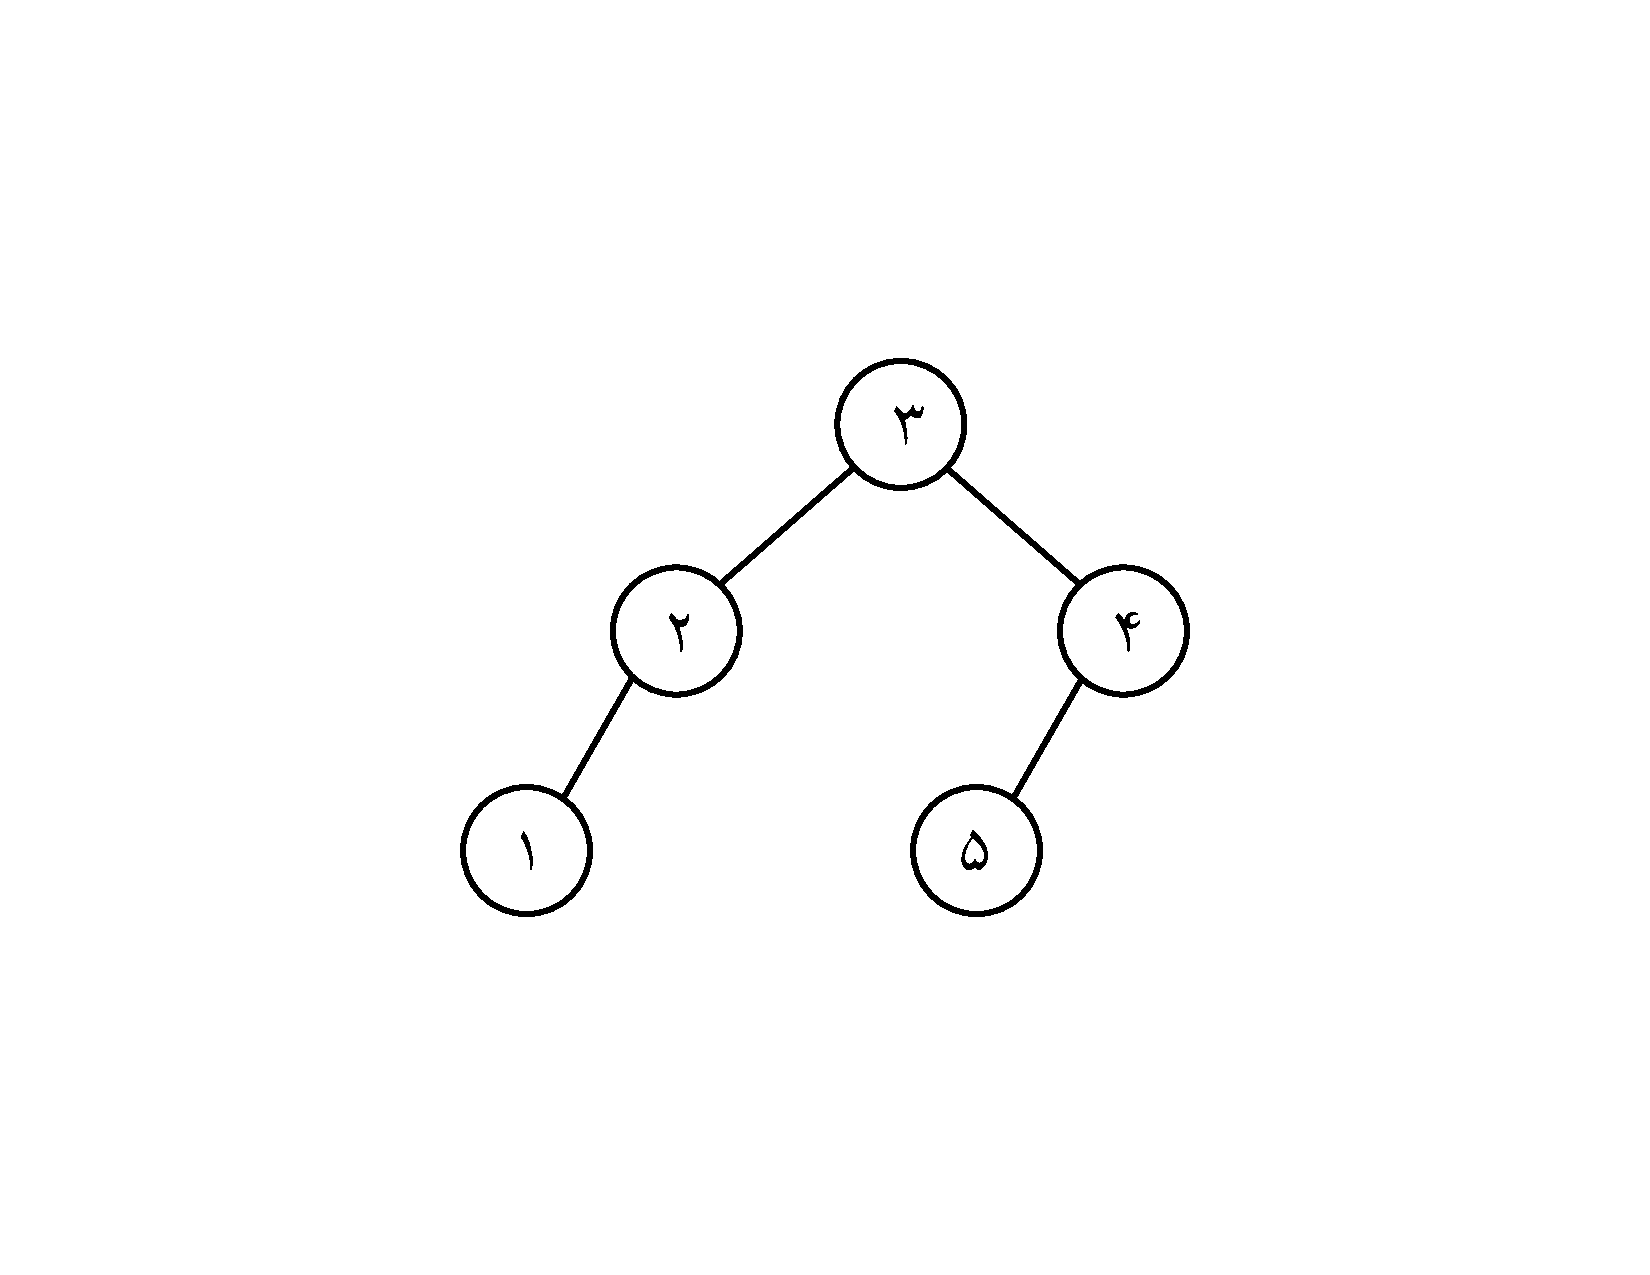
\includegraphics[scale=0.36]{figs/ch5/median_priority_queue_1.pdf}
\caption{داده‌ساختار صف اولویت میانه که در آن عنصر میانه در ریشه درخت دودویی قرار دارد}\label{ch5:fig:medPrioQueue1}
\end{center}
\end{figure}

می‌توانیم عنصر میانه را در یکی از دو درخت هیپ نیز قرار دهیم. برای مثال اگر عنصر میانه را در هیپ بیشینه قرار دهیم داده‌ساختار صف اولویت میانه مانند آنچه در شکل {\eqref{ch5:fig:medPrioQueue2}} نشان داده شده است خواهد بود.

\begin{figure}
\begin{center}
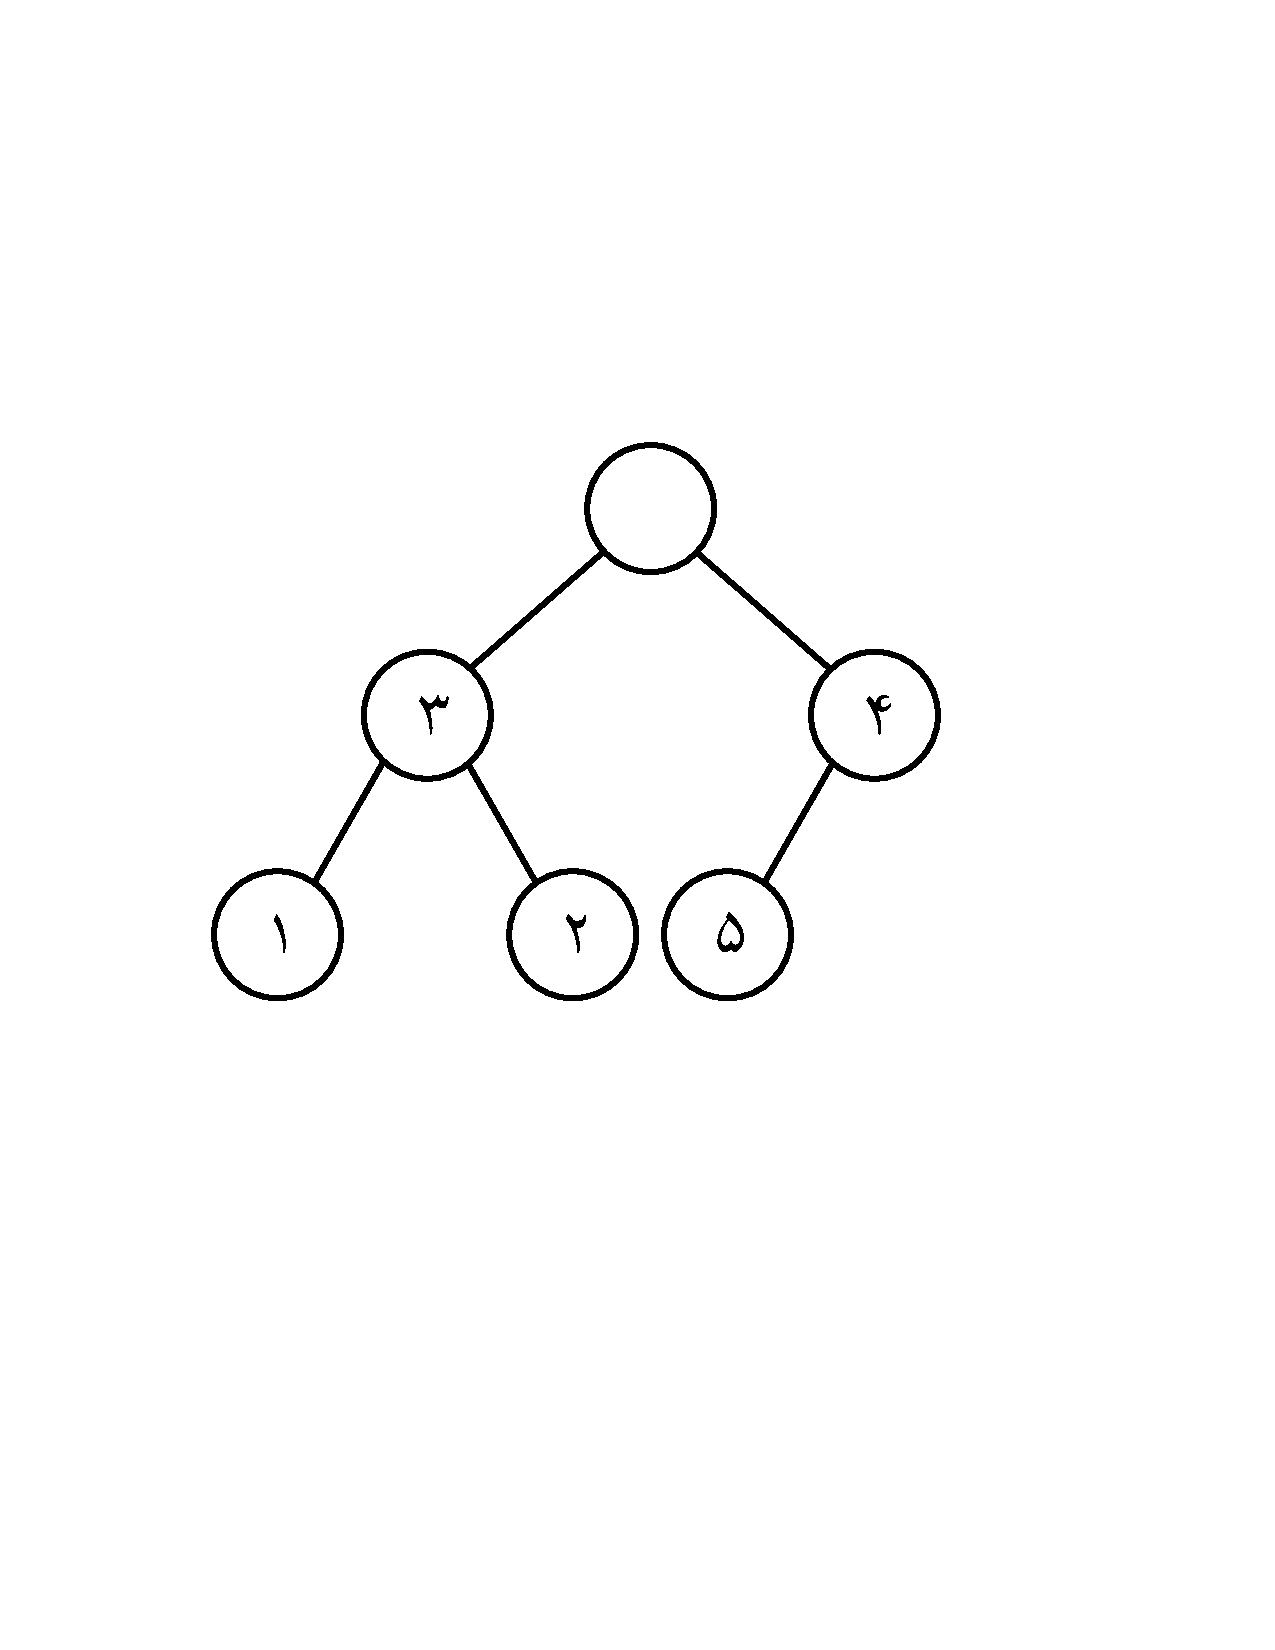
\includegraphics[scale=0.36]{figs/ch5/median_priority_queue_2.pdf}
\caption{داده‌ساختار صف اولویت میانه که در آن عنصر میانه در ریشه زیردرخت چپ درخت دودویی قرار دارد}\label{ch5:fig:medPrioQueue2}
\end{center}
\end{figure}

در ادامه فرض می‌کنیم که از حالت ذخیره‌سازی دوم استفاده شده است. با این روش پیاده‌سازی، برای حذف عنصر میانه، در شرایطی که تعداد عناصر هیپ بیشینه و هیپ کمینه با یکدیگر برابر نباشند، همواره عنصر ریشه‌ی درختی که تعداد عناصرش یکی بیشتر از دیگری است را به عنوان میانه جدید انتخاب می‌کنیم. اما اگر تعداد عناصر هر دو هیپ با یکدیگر برابر باشند می‌توان به دلخواه هر یک از دو ریشه‌ی هیپ‌های مذکور را به عنوان میانه‌ی جدید انتخاب کرد. 

در ادامه بدین صورت قرارداد می‌کنیم که اگر تعداد عناصر هر دو هیپ با یکدیگر برابر بودند آنگاه عنصر ریشه هیپ بیشینه به عنوان میانه جدید در نظر گرفته خواهد شد. در ادامه الگوریتم‌های مربوط به اعمال درج و حذف را شرح داده و نشان می‌دهیم که هر دو از مرتبه {$O(\lg n)$} هستند.

برای حذف عنصر میانه در ابتدا باید بررسی کنیم که هر کدام از دو درخت هیپ‌ دارای چه تعداد عنصر هستند. برای این کار می‌توان از دو متغیر استفاده کرد که هر کدام تعداد عناصر یکی از هیپ‌ها را نگه می‌دارد. اگر تعداد عناصر دو هیپ‌ با یکدیگر برابر نبود، کافیست ریشه‌ی درخت هیپی که یک عنصر بیشتر دارد را به عنوان  میانه‌ی جدید برگزینیم و آن ریشه را از هیپ حذف کنیم که در این صورت تعداد عناصر در هر دو هیپ با یکدیگر برابر خواهد شد. اما در صورتی که تعداد عناصر در هر دو هیپ با یکدیگر برابر باشد آنگاه عنصر ریشه هیپ بیشینه به عنوان میانه جدید در نظر گرفته می‌شود و این عنصر از درخت هیپ بیشینه حذف می‌شود. همانطور که می‌دانیم مرتبه زمانی عمل حذف یک عنصر از یک هیپ {$n$} عنصری برابر با {$O(\lg n)$} است. اگر تعداد عناصر هیپ بیشینه را {$n_1$} و تعداد عناصر هیپ کمینه را {$n_2$} در نظر بگیریم آنگاه حذف ریشه از هیپ بیشینه از مرتبه {$O(\lg n_1)$} و حذف ریشه از هیپ کمینه از مرتبه‌ {$O(\lg n_2)$} است. از طرفی می‌دانیم که {$n=n_1+n_2$} و  اختلاف {$n_1$} و {$n_2$} حداکثر یک واحد است. پس می‌توان گفت که حذف ریشه از هر کدام از درخت‌ها از مرتبه {$O(\lg (n/2))$} است که این نیز برابر با {$O(\lg n)$} است.

در هنگام درج در این داده‌ساختار باید کاری کرد که اختلاف تعداد عناصر هیپ‌های کمینه و بیشینه حداکثر یک باشد. در ادامه مقداری که قرار است درج شود را {$a$}، عنصر ریشه هیپ بیشینه را {$x$} و عنصر ریشه هیپ کمینه را {$y$} می‌نامیم. {$a$} را با {$x$} و {$y$} مقایسه می‌کنیم. سه حالت ممکن به شرح زیر خواهند بود:
\شروع{شمارش}
\فقره {$y \leq a$}: در این صورت {$a$} باید در هیپ کمینه، که شامل عناصر بزرگتر از میانه است، درج شود. اگر تعداد عناصر  هیپ کمینه، کمتر یا مساوی تعداد عناصر هیپ بیشینه باشد، عمل درج را به راحتی انجام می‌دهیم. در چنین حالتی تعداد عناصر هیپ کمینه برابر یا یکی بیشتر از عناصر هیپ بیشینه خواهد شد. اما در صورتی‌ که تعداد عناصر هیپ کمینه یکی بیشتر از هیپ بیشینه باشد، درج عنصر جدید در هیپ کمینه سبب خواهد شد که تعداد عناصر این هیپ دو واحد بیشتر از تعداد عناصر هیپ بیشینه شود که چنین حالتی قابل قبول نخواهد بود. در نتیجه پیش از درج عنصر جدید در هیپ کمینه، ابتدا ریشه‌ی هیپ کمینه، یعنی {$y$}، را حذف کرده و مقدار حذف شده را در هیپ بیشینه درج می‌کنیم. سپس {$a$} را در هیپ کمینه درج می‌کنیم که با انجام این کار دوباره اختلاف حداکثر یک واحدی تعداد عناصر دو هیپ نسبت به یکدیگر حفظ خواهد شد.

\فقره {$a \leq x$}: مراحل کلی عمل درج شبیه به حالت قبل است با این تفاوت که درج در هیپ بیشینه انجام خواهد شد.

\فقره {$y \leq a \leq x$}: در این حالت تعداد عناصر هیپ‌های بیشینه و کمینه را با یکدیگر مقایسه می‌کنیم. اگر تعداد عناصر هر دو هیپ برابر بود، می‌توان عمل درج را در هر یک از هیپ‌ها انجام داد. اما اگر تعداد عناصر دو هیپ یکسان نبود، درج را در هیپ با تعداد عناصر کمتر انجام می‌دهیم.
\پایان{شمارش}
با توجه به توضیحات ارائه ‌شده، برای درج یک عنصر در صف اولویت میانه در بدترین حالت باید یک عمل حذف و دو عمل درج در هیپ انجام داد. در نتیجه مرتبه زمانی عمل درج در بدترین حالت برابر با {$O(3\times \lg (n/2))$} است که این نیز از مرتبه‌ی {$O(\lg n)$} است.

\سوال درستی عبارت زیر را اثبات کنید.
\begin{quote}
\علامت‌راست‌نقل‌قول‌پارسی تعداد گره‌های با ارتفاع {$h$} در یک درخت هیپ {$n$} عنصری، حداکثر برابر با {$\lceil n/2^{h+1}\rceil$} است\علامت‌چپ‌نقل‌قول‌پارسی
\end{quote}

\پاسخ

اثبات را با استقرا بر روی {$h$} انجام می‌دهیم.

پایه‌ی استقرا: باید نشان دهیم هنگامی که {$h=0$} است تعداد گره‌های با ارتفاع {$h$}، کمتر یا مساوی {$\lceil n/2^{h+1}\rceil$} است. به عبارت دیگر باید نشان دهیم تعداد گره‌های با ارتفاع {$h=0$} کوچکتر یا مساوی {$\lceil n/2\rceil$} است.

اگر فرض کنیم درخت هیپ دارای عمق {$D$} است آنگاه گره‌های با ارتفاع صفر، که همان گره‌های برگ هستند، می‌توانند در عمق {$D$} یا {$D-1$} باشند و هر یک از این گره‌ها در یکی از دو حالت زیر صدق می‌کنند:
\شروع{فقرات}
\فقره گره‌‌ در عمق {$D$} قرار دارد.
\فقره گره‌ در عمق {$D-1$} قرار دارد و این گره پدر هیچ گره‌ای در عمق {$D$} نیست.
\پایان{فقرات}
حال فرض می‌کنیم {$x$}  تعداد گره‌های موجود در عمق {$D$} باشد. اگر {$n$} را تعداد کل گره‌های درخت در نظر بگیریم آنگاه {$n-x$} عددی فرد است زیرا {$n-x$} گره‌ی موجود، تشکیل یک درخت دودویی با حداکثر تعداد گره را می‌دهند. به عبارت دیگر با نادیده گرفتن {$x$} گره‌ی موجود در عمق {$D$} دارای درختی کامل با {$n-x$} گره خواهیم بود. به این ترتیب می‌توان تعداد گره‌ها‌ی درخت را برابر با {$n=(2^{D}-1)+x$} در نظر گرفت. با توجه به فرد بودن مقدار {$n-x$}، اگر {$n$} فرد باشد آنگاه {$x$} زوج است و اگر {$n$} زوج باشد {$x$} فرد است.

برای اثبات پایه‌ی استقرا باید دو حالت زوج و فرد بودن {$n$} را به صورت جداگانه درنظر بگیریم. برای ادامه‌ی اثبات توجه داشته باشید که در عمق {$d$} به شرطی که {$d<D$} باشد دارای {$2^d$} گره هستیم زیرا درخت در چنین عمقی دارای حداکثر تعداد گره است.

اگر {$n$} فرد باشد آنگاه {$x$} زوج است. چون {$x$} زوج است پس دقیقاً {$x/2$} گره در عمق {$D-1$} قرار دارند که والدین {$x$} گره‌ی موجود در عمق {$D$} هستند. این بدین معنی است که تعداد گره‌های عمق {$D-1$} که پدر هیچ گره‌ای در عمق {$D$} نیستند برابر است با:
\begin{equation}
2^{D-1}-\frac{x}{2}
\end{equation}
این یعنی علاوه بر {$x$} گره‌ی برگ موجود در عمق {$D$} دارای {$2^{D-1}-x/2$} گره برگ در عمق {$D-1$} نیز هستیم. پس تعداد کل گره‌های برگ برابر خواهد بود با {$x+(2^{D-1}-x/2)$} که این مقدار معادل با {$2^{D-1}+x/2$} است. این مقدار را می‌توان به صورت {$(2^D+x)/2$} نیز نوشت. با توجه به اینکه {$x$} زوج است مقدار {$(2^D+x)/2$} معادل با {$\lceil (2^D+x-1)/2\rceil$} است. حال اگر به جای عبارت {$2^D+x-1$} مقدار معادل آن یعنی {$n$} را جایگزین کنیم آنگاه عبارت {$\lceil (2^D+x-1)/2\rceil$} تبدیل به {$\lceil n/2\rceil$} می‌شود. بدین ترتیب نشان دادیم که وقتی {$n$} فرد است تعداد گره‌های با عمق صفر برابر با {$\lceil n/2\rceil$} است.

حال اگر فرض کنیم {$n$} زوج است آنگاه {$x$} فرد خواهد بود و با استدلالی شبیه به استدلال انجام شده در حالت فرد بودن {$n$}، تعداد گره‌های با عمق صفر به صورت زیر به دست می‌آید:
\begin{align}
n_0 &= x+\left( 2^{D-1} + \frac{x+1}{2}\right)\nonumber\\
&=2^{D-1}+\frac{x-1}{2}\nonumber\\
&=\frac{2^{D-1}-1+x}{2}\nonumber\\
&=\frac{n}{2}\label{ch5:eqn:BaseCaseEvenN}
\end{align}
چون {$n$} زوج است در نتیجه می‌توان تساوی {\eqref{ch5:eqn:BaseCaseEvenN}} را معادل با {$n_0=\lceil n/2\rceil$} در نظر گرفت. به این ترتیب نشان دادیم وقتی {$n$} زوج باشد تعداد گره‌های با ارتفاع صفر برابر با {$\lceil n/2\rceil$} است.

با توجه به اینکه هم برای {$n$} فرد و هم برای {$n$} زوج نشان دادیم که تعداد گره‌های برگ در ارتفاع صفر حداکثر برابر با {$\lceil n/2\rceil$} است در نتیجه می‌توان گفت پایه‌ی استقرا برقرار است.

فرض استقرا: فرض می‌کنیم در یک درخت هیپ حداکثر تعداد گره‌های برگ با ارتفاع {$h-1$} برابر با {$\lceil n/2^{h}\rceil$} است.

حکم استقرا: نشان می‌دهیم در یک درخت هیپ حداکثر تعداد گره‌های برگ با ارتفاع {$h$} برابر با {$\lceil n/2^{h+1}\rceil$} است.

فرض می‌کنیم {$n_h$} تعداد گره‌های برگ با عمق {$h$} در یک درخت هیپ {$n$} عنصری به نام {$T$} باشد. {$T'$} را درختی در نظر می‌گیریم که با حذف برگ‌های درخت {$T$} حاصل شده است. به این ترتیب تعداد گره‌های درخت {$T'$}، که آن را با {$n'$} نشان می‌دهیم، برابر است با {$n'=n-n_0$}. با توجه به اثباتی که برای پایه‌ی استقرا انجام دادیم می‌دانیم که {$n_0=\lceil n/2 \rceil$} است. پس مقدار {$n'$} را می‌توان به صورت زیر نوشت:
\begin{displaymath}
n' = n - n_0=n-\left\lceil \frac{n}{2}\right\rceil =\left\lfloor \frac{n}{2}\right\rfloor
\end{displaymath}
توجه به این نکته ضروری است که اگر ارتفاع گره‌ای در درخت {$T$} برابر با {$h$} باشد آنگاه چنین گره‌ای در درخت {$T'$} دارای ارتفاع {$h-1$} است. با توجه به این نکته و تعریف {${n'}_{h-1}$} به ‌عنوان تعداد گره‌های با ارتفاع {$h-1$} در درخت {$T'$} می‌توان گفت {$n_h=n'_{h-1}$}. حال با استفاده از فرض استقرا داریم:
\begin{displaymath}
n_h=n'_{h-1} \leq \left\lceil \frac{n'}{2^h}\right\rceil=\left\lceil \frac{\left\lfloor n/2 \right\rfloor}{2^h}\right\rceil \leq \left\lceil \frac{n/2}{2^h}\right\rceil=\left\lceil \frac{n}{2^{h+1}} \right\rceil
\end{displaymath}
بدین ترتیب اثبات کامل است.